% Aberdeen style guide should be followed when using this
% layout. Their template powerpoint slide is used to extract the
% Aberdeen color and logo but is otherwise ignored (it has little or
% no formatting in it anyway).
%
% http://www.abdn.ac.uk/documents/style-guide.pdf

%%%%%%%%%%%%%%%%%%%% Document Class Settings %%%%%%%%%%%%%%%%%%%%%%%%%
% Pick if you want slides, or draft slides (no animations)
%%%%%%%%%%%%%%%%%%%%%%%%%%%%%%%%%%%%%%%%%%%%%%%%%%%%%%%%%%%%%%%%%%%%%%
%Normal document mode
\documentclass[10pt,compress]{beamer}
%Draft or handout mode
%\documentclass[10pt,compress,handout]{beamer}
%\documentclass[10pt,compress,handout,ignorenonframetext]{beamer}
\newcommand{\frc}{\displaystyle\frac}


%%%%%%%%%%%%%%%%%%%% General Document settings %%%%%%%%%%%%%%%%%%%%%%%
% These settings must be set for each presentation
%%%%%%%%%%%%%%%%%%%%%%%%%%%%%%%%%%%%%%%%%%%%%%%%%%%%%%%%%%%%%%%%%%%%%%


\newcommand{\shortname}{Dr Jeff Gomes}
\newcommand{\fullname}{Dr Jeff Gomes}
\institute{School of Engineering}
\newcommand{\emailaddress}{jefferson.gomes@abdn.ac.uk}
\newcommand{\logoimage}{../FigBanner/UoAHorizBanner}
\title{Engineering Thermodynamics (EG3521)}
\subtitle{Module 3: Refrigeration $\&$ Liquefaction}
\date[11-13/03/2014]{11-13 March 2014}

%%%%%%%%%%%%%%%%%%%% Template settings %%%%%%%%%%%%%%%%%%%%%%%%%%%%%%%
% You shouldn't have to change below this line, unless you want to.
%%%%%%%%%%%%%%%%%%%%%%%%%%%%%%%%%%%%%%%%%%%%%%%%%%%%%%%%%%%%%%%%%%%%%%
\usecolortheme{whale}
\useoutertheme{infolines}

% Use the fading effect for items that are covered on the current
% slide.
\beamertemplatetransparentcovered

% We abuse the author command to place all of the slide information on
% the title page.
\author[\shortname]{%
  \fullname\\\ttfamily{\emailaddress}
}


%At the start of every section, put a slide indicating the contents of the current section.
%\AtBeginSection[] {
%  \begin{frame}
%    \frametitle{Section Outline}
%    \tableofcontents[currentsection]
%  \end{frame}
%}

% Allow the inclusion of movies into the Presentation! At present,
% only the Okular program is capable of playing the movies *IN* the
% presentation.
\usepackage{multimedia}
\usepackage{animate}

%%%%% Color settings
\usepackage{color}
%% The background color for code listings (i.e. example programs)
\definecolor{lbcolor}{rgb}{0.9,0.9,0.9}%
\definecolor{UoARed}{rgb}{0.64706, 0.0, 0.12941}
\definecolor{UoALight}{rgb}{0.85, 0.85, 0.85}
\definecolor{UoALighter}{rgb}{0.92, 0.92, 0.92}
\setbeamercolor{structure}{fg=UoARed} % General background and higlight color
\setbeamercolor{frametitle}{bg=black} % General color
\setbeamercolor{frametitle right}{bg=black} % General color
\setbeamercolor{block body}{bg=UoALighter} % For blocks
\setbeamercolor{structure}{bg=UoALight} % For blocks
% Rounded boxes for blocks
\setbeamertemplate{blocks}[rounded]

%%%%% Font settings
% Aberdeen requires the use of Arial in slides. We can use the
% Helvetica font as its widely available like so
% \usepackage{helvet}
% \renewcommand{\familydefault}{\sfdefault}
% But beamer already uses a sans font, so we will stick with that.

% The size of the font used for the code listings.
\newcommand{\goodsize}{\fontsize{6}{7}\selectfont}

% Extra math packages, symbols and colors. If you're using Latex you
% must be using it for formatting the math!
\usepackage{amscd,amssymb} \usepackage{amsfonts}
\usepackage[mathscr]{eucal} \usepackage{mathrsfs}
\usepackage{latexsym} \usepackage{amsmath} \usepackage{bm}
\usepackage{amsthm} \usepackage{textcomp} \usepackage{eurosym}
% This package provides \cancel{a} and \cancelto{a}{b} to "cancel"
% expressions in math.
\usepackage{cancel}

% Get rid of font warnings as modern LaTaX installations have scalable
% fonts
\usepackage{type1cm} 

%\usepackage{enumitem} % continuous numbering throughout enumerate commands

% For exact placement of images/text on the cover page
\usepackage[absolute]{textpos}
\setlength{\TPHorizModule}{1mm}%sets the textpos unit
\setlength{\TPVertModule}{\TPHorizModule} 

% Source code formatting package
\usepackage{listings}%
\lstset{ backgroundcolor=\color{lbcolor}, tabsize=4,
  numberstyle=\tiny, rulecolor=, language=C++, basicstyle=\goodsize,
  upquote=true, aboveskip={1.5\baselineskip}, columns=fixed,
  showstringspaces=false, extendedchars=true, breaklines=false,
  prebreak = \raisebox{0ex}[0ex][0ex]{\ensuremath{\hookleftarrow}},
  frame=single, showtabs=false, showspaces=false,
  showstringspaces=false, identifierstyle=\ttfamily,
  keywordstyle=\color[rgb]{0,0,1},
  commentstyle=\color[rgb]{0.133,0.545,0.133},
  stringstyle=\color[rgb]{0.627,0.126,0.941}}

% Allows the inclusion of other PDF's into the final PDF. Great for
% attaching tutorial sheets etc.
\usepackage{pdfpages}
\setbeamercolor{background canvas}{bg=}  

% Remove foot note horizontal rules, they occupy too much space on the slide
\renewcommand{\footnoterule}{}

% Force the driver to fix the colors on PDF's which include mixed
% colorspaces and transparency.
\pdfpageattr {/Group << /S /Transparency /I true /CS /DeviceRGB>>}

% Include a graphics, reserve space for it but
% show it on the next frame.
% Parameters:
% #1 Which slide you want it on
% #2 Previous slides
% #3 Options to \includegraphics (optional)
% #4 Name of graphic
\newcommand{\reserveandshow}[4]{%
\phantom{\includegraphics<#2|handout:0>[#3]{#4}}%
\includegraphics<#1>[#3]{#4}%
}

\begin{document}

% Title page layout
\begin{frame}
  \titlepage
  \vfill%
  \begin{center}
    \includegraphics[clip,width=0.8\textwidth]{\logoimage}
  \end{center}
\end{frame}

% Table of contents
%\frame{ \frametitle{Slides Outline}
%  \tableofcontents
%}


%%%%%%%%%%%%%%%%%%%% The Presentation Proper %%%%%%%%%%%%%%%%%%%%%%%%%
% Fill below this line with \begin{frame} commands! It's best to
% always add the fragile option in case you're going to use the
% verbatim environment.
%%%%%%%%%%%%%%%%%%%%%%%%%%%%%%%%%%%%%%%%%%%%%%%%%%%%%%%%%%%%%%%%%%%%%%

\section{Absorption Refrigeration Cycle}

\subsection{Intended Learning Objectives}
%%%
%%% Slide
%%%
\begin{frame}
 \frametitle{Introduction}
  In Module 3, we will cover the following topics:
  \begin{enumerate}[(i)]
   \item <1-> Fundamentals of Refrigeration: Refrigeration and heat pump; Elements of refrigeration; Efficieny; Classification and Properties of Refrigerants;
   \item <1-> Gas-Refrigeration Systems: Reversed Carnot, Brayton and Stirling cycles;
   \item <1-> Analysis of Air-Conditioning Processes and;
   \item <1-> Vapour-Refrigeration Systems: Ideal and Actual Vapour-Compression Refrigeration Cycles; Criteria for choosing Refrigerant Fluids; Cascade and Multi-stage Vapour-Compression systems;
   \item <2-> \textcolor{blue}{Absorption Refrigeration Systems;}
   \item <3-> \textcolor{blue}{Liquefaction Processes: Claude and Linde Cycles.}
  \end{enumerate}
\end{frame}

%%%
%%% Slide
%%%
\begin{frame}
 \frametitle{Aims and Objectives}
  \begin{enumerate}[(i)]
   \item <1-> Introduce vapour absorption refrigeration cycles (VARC);
   \item <2-> Explain basic principles of VARC and compare it with vapour-compression refrigeration cycles;
   \item <3-> Describe single-stage VARC with the associated thermal analysis.
  \end{enumerate}
\end{frame}

%%%
%%% Slide
%%%
\begin{frame}
 \frametitle{Aims and Objectives}
  At the end of this Module, you should be able to:
  \begin{enumerate}[(i)]
   \item <1-> Identify elements of vapour absorption refrigeration cycles;
   \item <2-> Identify refrigerant fluids properties for VARCs;
   \item <3-> Solve problems based on the vapour absorption refrigeration cycles.
  \end{enumerate}
\end{frame}


\subsection{Bibliography} 
%%%
%%% Slide
%%%
\begin{frame}
 \frametitle{Suggested References}
  Literature relevant for this module:
  \begin{enumerate}[(a)]
   \item J.M. Smith, H.C. Van Ness and M.M. Abbott, $\lq$Introduction to Chemical Engineering Thermodynamics', 6$^{th}$ Edition: Chapter 9.4-6;
   %\item I. Muller and W.H. Muller, $\lq$Fundamentals of Thermodynamics and Applications' (2009) Chapter 6.3;
   \item Y.A. Cengel and M.A. Boles, $\lq$Thermodynamics -- An Engineering Approach' , 5$^{th}$ Edition: Chapters 11.7,9;
   %\item E. Logan, $\lq$Thermodynamics -- Processes and Applications' (1999): 8.2-3;
   \item M.J. Moran, H.J. Shapiro, D.D. Boettner, M.B. Bailey, $\lq$Principles of Engineering Thermodynamics', 7$^{th}$ Edition: Chapters: 10.5,6;
   \item R.T. Balmer, $\lq$Modern Engineering Thermodynamics' (2011) Chapters: 14.10;
   %\item \href{http://www.sfsb.unios.hr/test/testhome/vtAnimations/animations/chapter09/refrigeration/index1.html}{\tiny{http://www.sfsb.unios.hr/test/testhome/vtAnimations/animations/chapter09/refrigeration/index1.html}}
  \end{enumerate}
\end{frame}


\subsection{Introduction}
%%%
%%% Slide
%%%
\begin{frame}
 \frametitle{Background}
  \begin{enumerate}[(a)]
   \item <1-> We studied that in \textcolor{blue}{vapour compression refrigeration cycles} the power input is realised by isentropically compressing the refrigerant fluid from low pressure to high pressure and;
   \item <2-> The \textcolor{blue}{COP} can be enhanced (for a given refrigeration capacity) by reducing the \textcolor{blue}{work input $\left(\dot{W}_{c}\right)$} into the system. However;
   \item <3-> If we want to reduce the work input in \textcolor{blue}{vapour absorption refrigeration cycles}, the \textcolor{red}{compressor} is replaced by a \textcolor{red}{pump} and the fluid is in the liquid phase;
   \item <4-> The \textcolor{blue}{average specific volume} of the \textcolor{blue}{\it liquid refrigerant} is much smaller than that if the refrigerant is in the \textcolor{blue}{\it vapour phase} $\Longrightarrow$ {\it Less work is required for increasing the pressure in the pump};
   \item <5-> \textcolor{blue}{VARCs} run on \textcolor{blue}{low-grade thermal energy}, therefore they are more often used when low-grade energy source (e.g., solar energy, geothermal energy, waste heat from co-generation etc) is available.
  \end{enumerate}
\end{frame}

%%%
%%% Slide
%%%
\begin{frame}
 \frametitle{Background -- Why the new Design?}
  \begin{columns}
   \begin{column}[c]{0.45\linewidth}
    \begin{figure}%
     \vbox{
      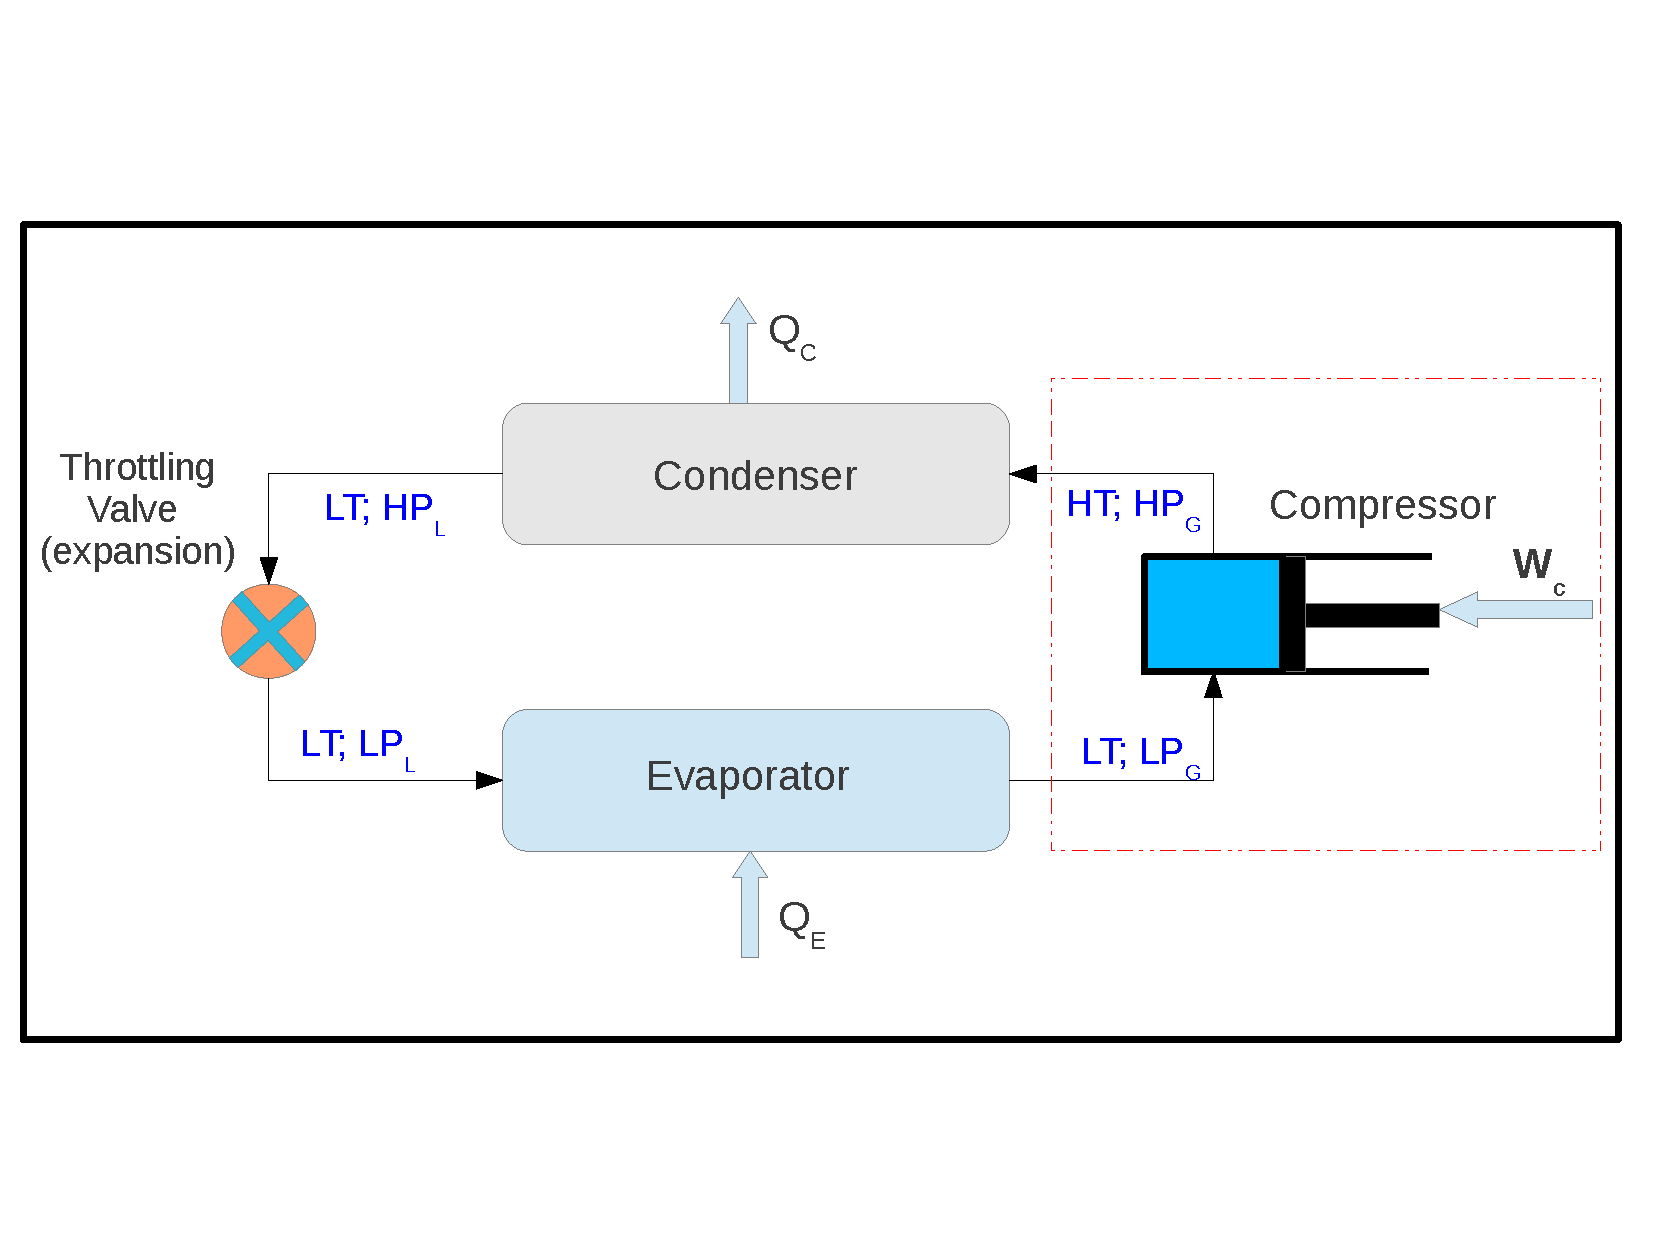
\includegraphics[width=5.5cm,clip]{./Pics/Overview_Refrig31}
      \vspace{-.5cm}
      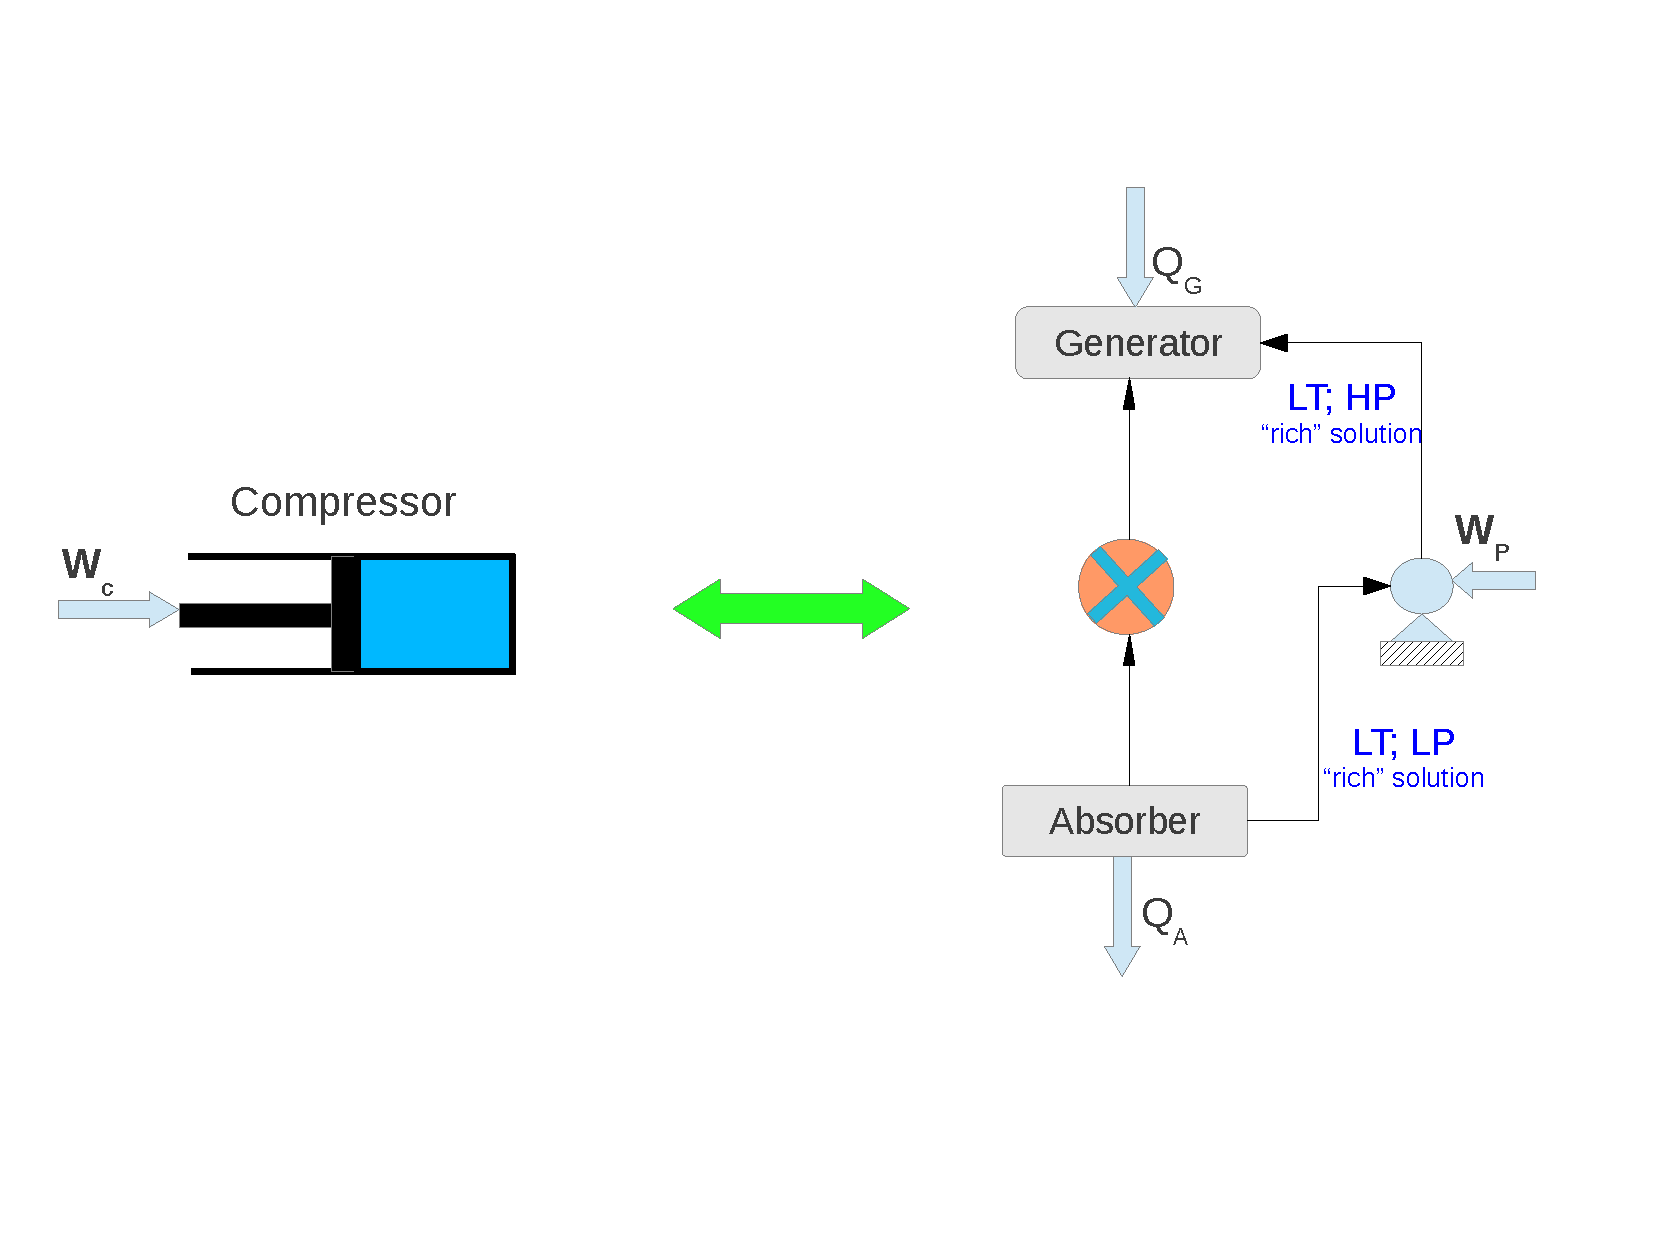
\includegraphics[width=5.5cm,clip]{./Pics/Overview_Refrig33}}
    \end{figure}  
   \end{column}  
   \begin{column}[c]{0.55\linewidth}
  \begin{enumerate}[(a)]
   \item <1-> The \textcolor{blue}{VARC} is based on using a pump to raise the pressure of the refrigerant fluid to take advantage of the smaller amount of work requirement;
   \item <2-> A liquid can be pumped \textcolor{blue}{\it more efficiently} than a vapour can be compressed;
   \item <3-> It involves the absorption of the refrigerant by a {\it transport medium} (or {\it carrier liquid} or {\it absorbent}) -- e.g., Ammonia (refrigerant) / Water (carrier/medium)
   \item <4-> The pressurised liquid is fed into a {\it generator} where the refrigerant vapour is boiled off at a much higher pressure;
  \end{enumerate}
   \end{column}  
 \end{columns}  
\end{frame}

%%%
%%% Slide
%%%
\begin{frame}
 \frametitle{Background -- Why the new Design?}
  \begin{columns}
   \begin{column}[c]{0.45\linewidth}
    \begin{figure}%
     \vbox{
      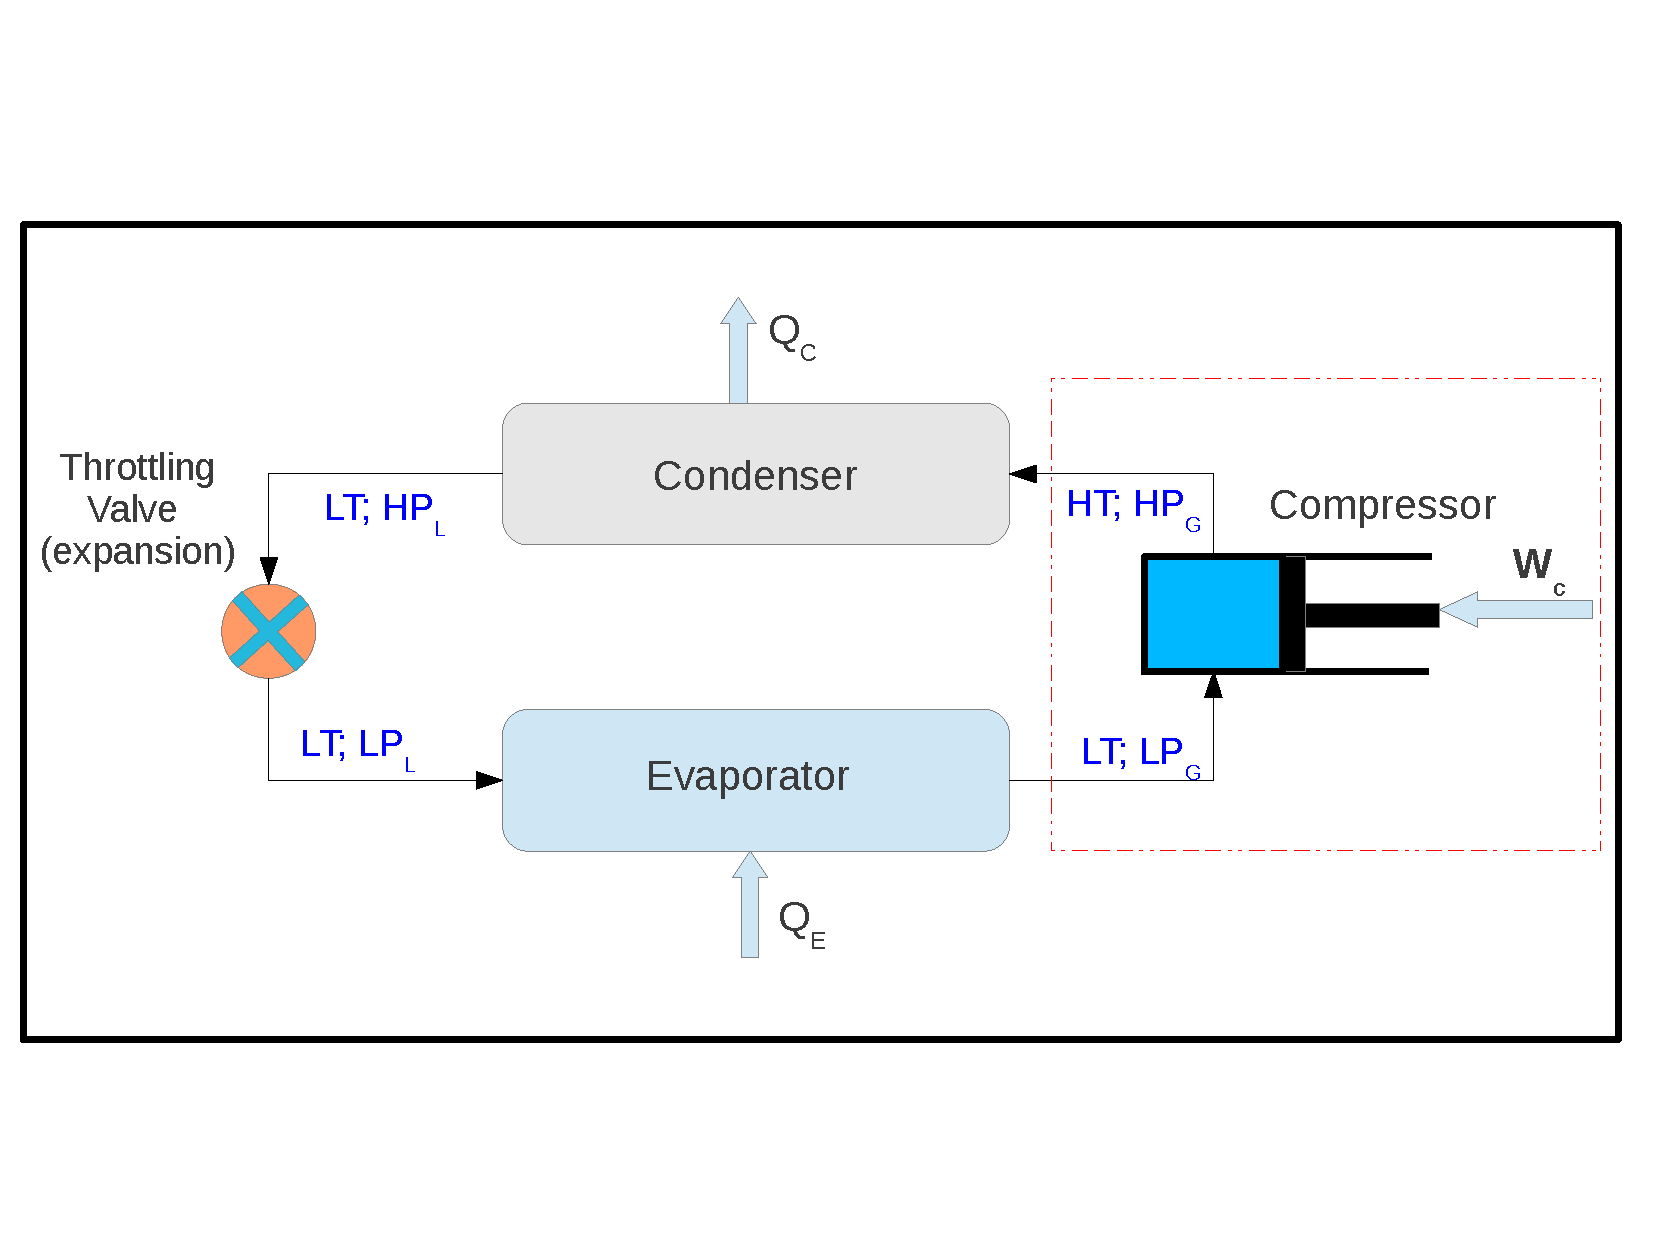
\includegraphics[width=5.5cm,clip]{./Pics/Overview_Refrig31}
      \vspace{-.5cm}
      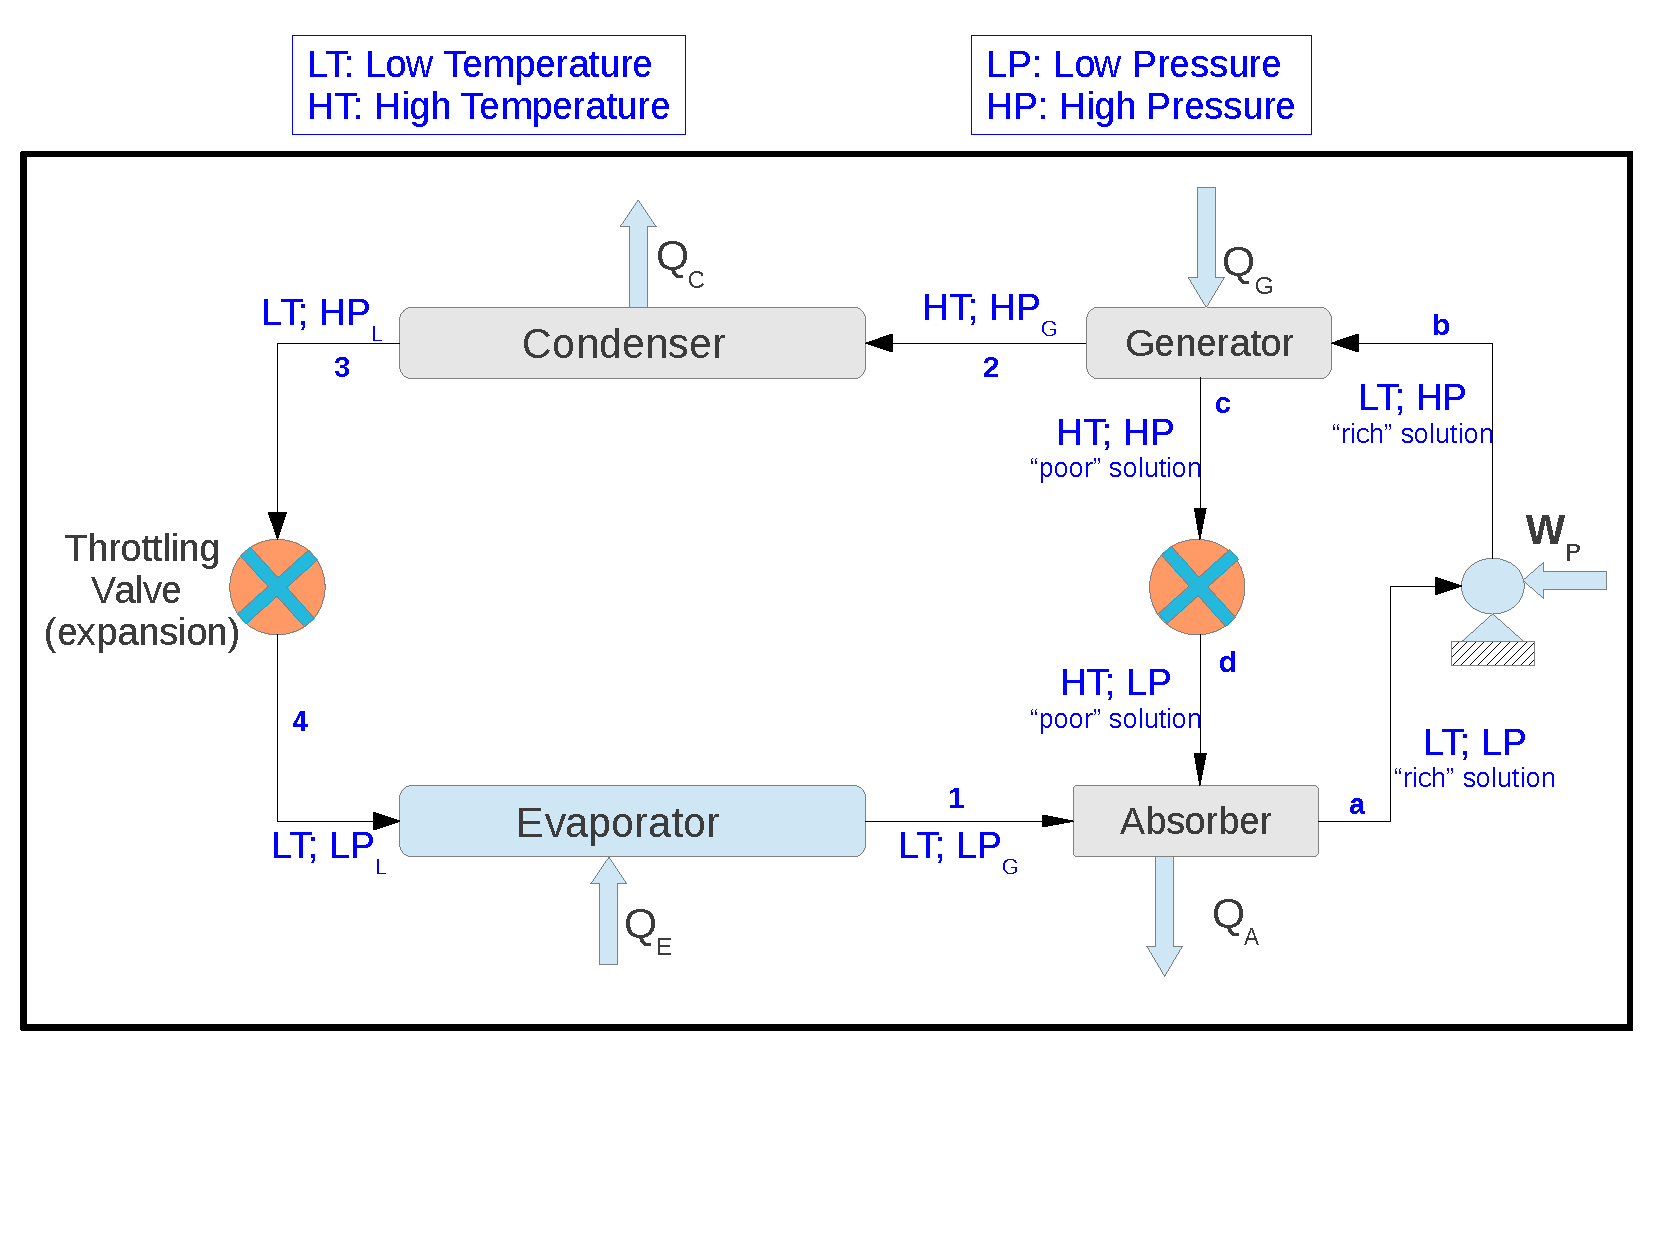
\includegraphics[width=5.5cm,clip]{./Pics/Overview_Refrig32}}
    \end{figure}  
   \end{column}  
   \begin{column}[c]{0.55\linewidth}
  \begin{enumerate}[(a)]
   \item <1-> The absorbent returns to the {\it absorber} to continue the process;
   \item <2-> the high-pressure refrigerant vapour continues the remainining of the reversed Rankine cycle. 
   \item <3-> \textcolor{blue}{Examples:} Ammonia (refrigerant) / Water (medium), Water (refrigerant) - Lithium Bromide (medium), Water (refrigerant) - Lithium Chloride (medium)
  \end{enumerate}
   \end{column}  
 \end{columns}  
\end{frame}

\subsection{Fundamentals}
%%%
%%% Slide
%%%
\begin{frame}
 \frametitle{Basic Principles -- Process Flow} 
  \begin{columns}
   \begin{column}[c]{0.45\linewidth}
    \begin{figure}%
     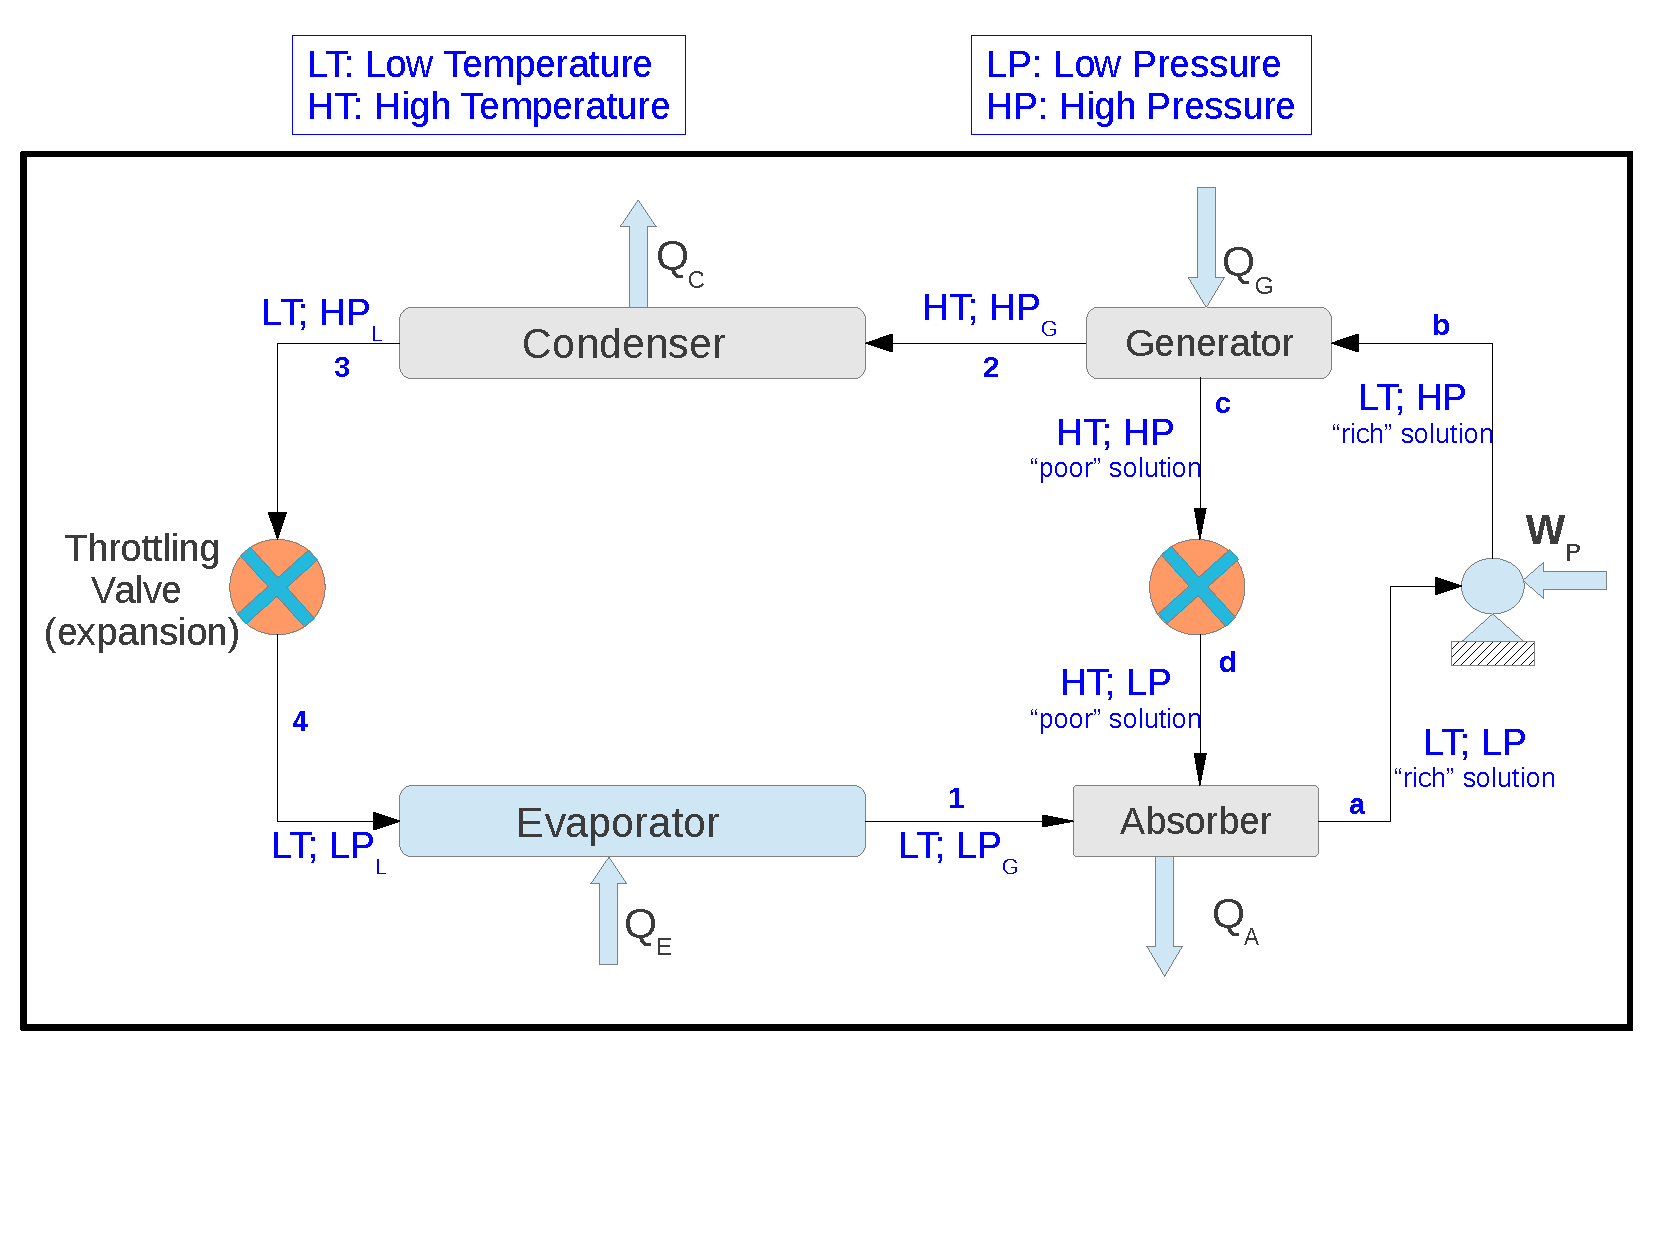
\includegraphics[width=5.5cm,clip]{./Pics/Overview_Refrig32}
    \end{figure}  
   \end{column}  
   \begin{column}[c]{0.55\linewidth}
    \begin{enumerate}[(a)]
     \item <1-> For simplicity let's assume a system involving \textcolor{blue}{Ammonia (as refrigerant fluid)} and \textcolor{blue}{Water (as absorbent)};
     \item <2-> The solubility of ammonia in water at \textcolor{blue}{{\it low T and P}} is higher than at \textcolor{blue}{{\it high T and P}};
     \item <3-> The \textcolor{blue}{ammonia (V)} that leaves the evaporator \textcolor{blue}{(1)} is \textcolor{blue}{absorbed in the LT {\it absorber} with rejection of heat};
   %\item <-> 
   \end{enumerate}
  \end{column}  
 \end{columns}  
\end{frame}

%%%
%%% Slide
%%%
\begin{frame}
 \frametitle{Basic Principles -- Process Flow} 
  \begin{columns}
   \begin{column}[c]{0.45\linewidth}
    \begin{figure}%
     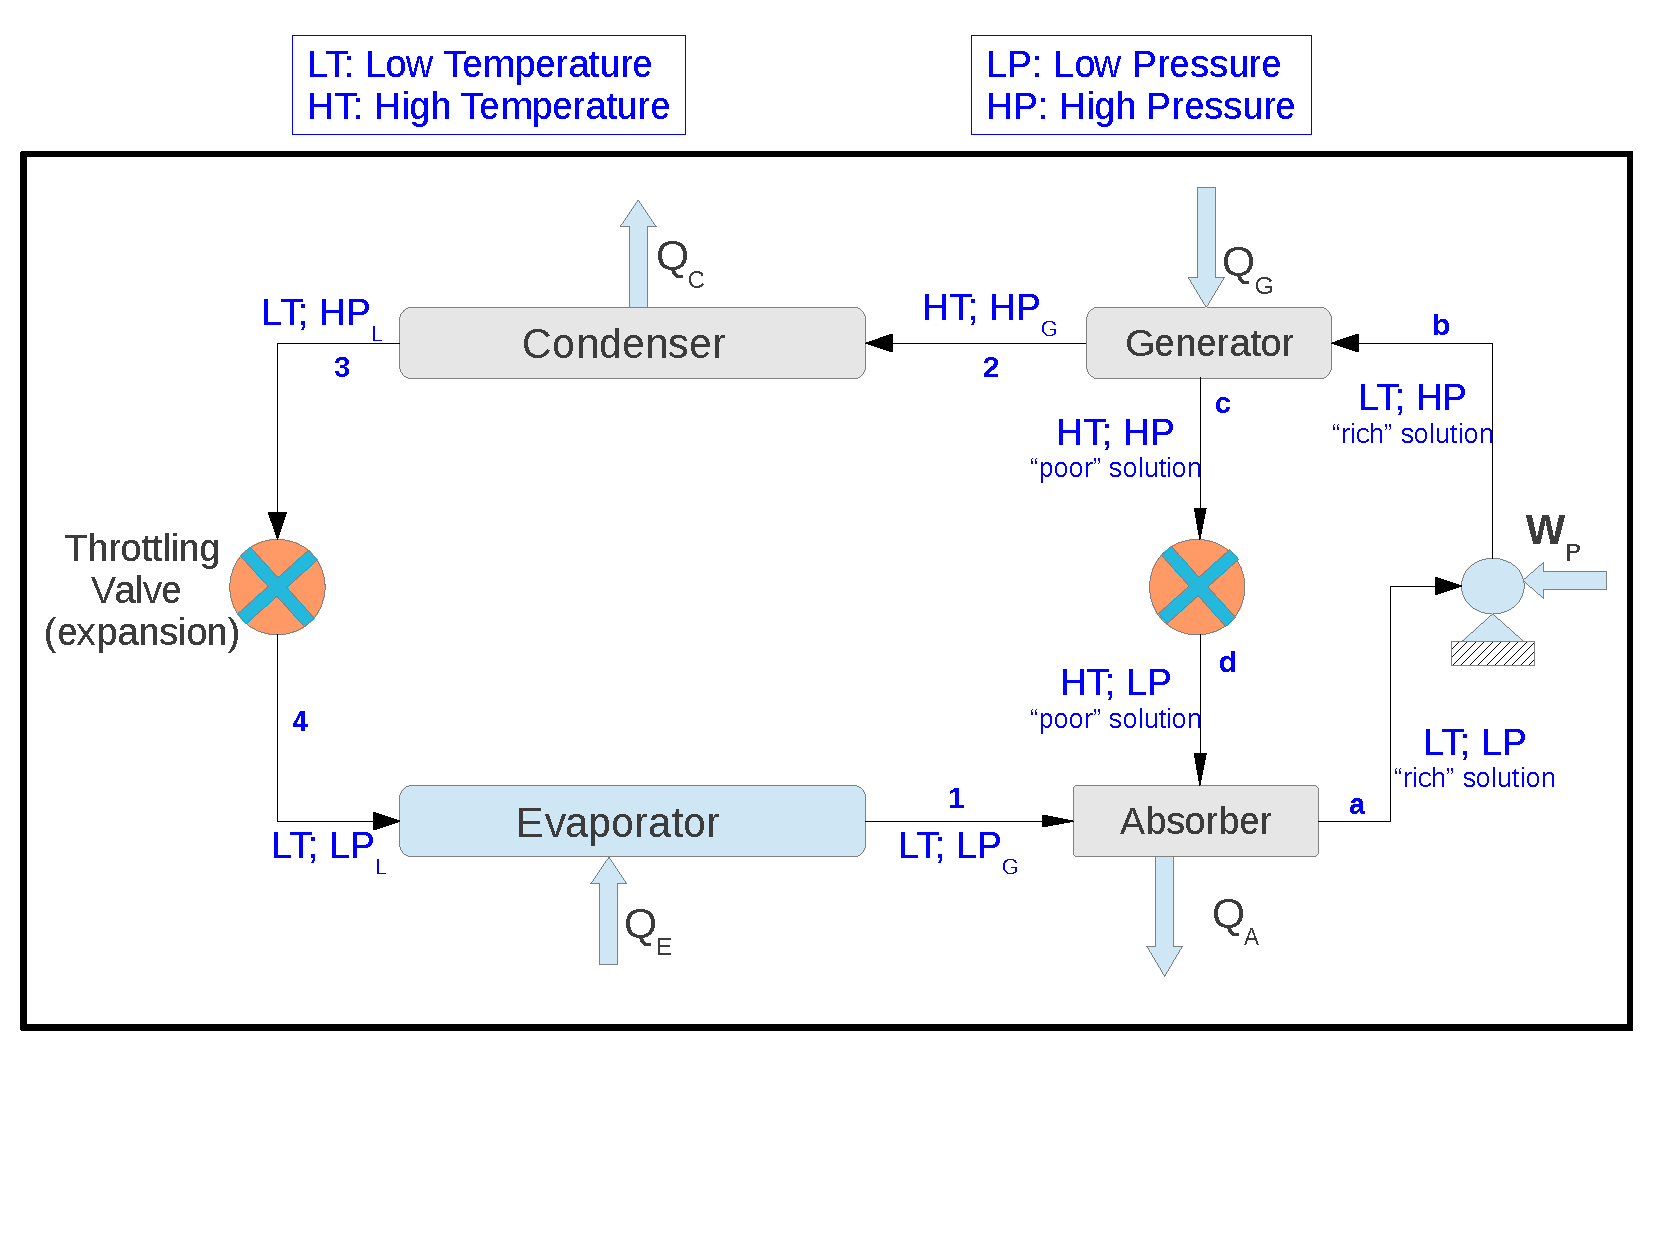
\includegraphics[width=5.5cm,clip]{./Pics/Overview_Refrig32}
    \end{figure}  
   \end{column}  
   \begin{column}[c]{0.55\linewidth}
    \begin{enumerate}[(a)]
     \item <1-> The resulting {\it ammonia + water} solution is then pumped to the higher pressure and heated in the generator;
     \item <2-> Because of the reduced solubility of the solution at {\it higher P and T}, the vapour is removed from the solution;
     \item <3-> The vapour is then driven to the condenser and the weakened ammonia in water solution is returned to the {\it absorber}.
   %\item <-> 
   \end{enumerate}
  \end{column}  
 \end{columns}  
\end{frame}

%%%
%%% Slide
%%%
\begin{frame}
 \frametitle{Basic Principles -- Phase Equilibrium Diagram} 
  \begin{columns}
   \begin{column}[c]{0.45\linewidth}
    \begin{figure}%
     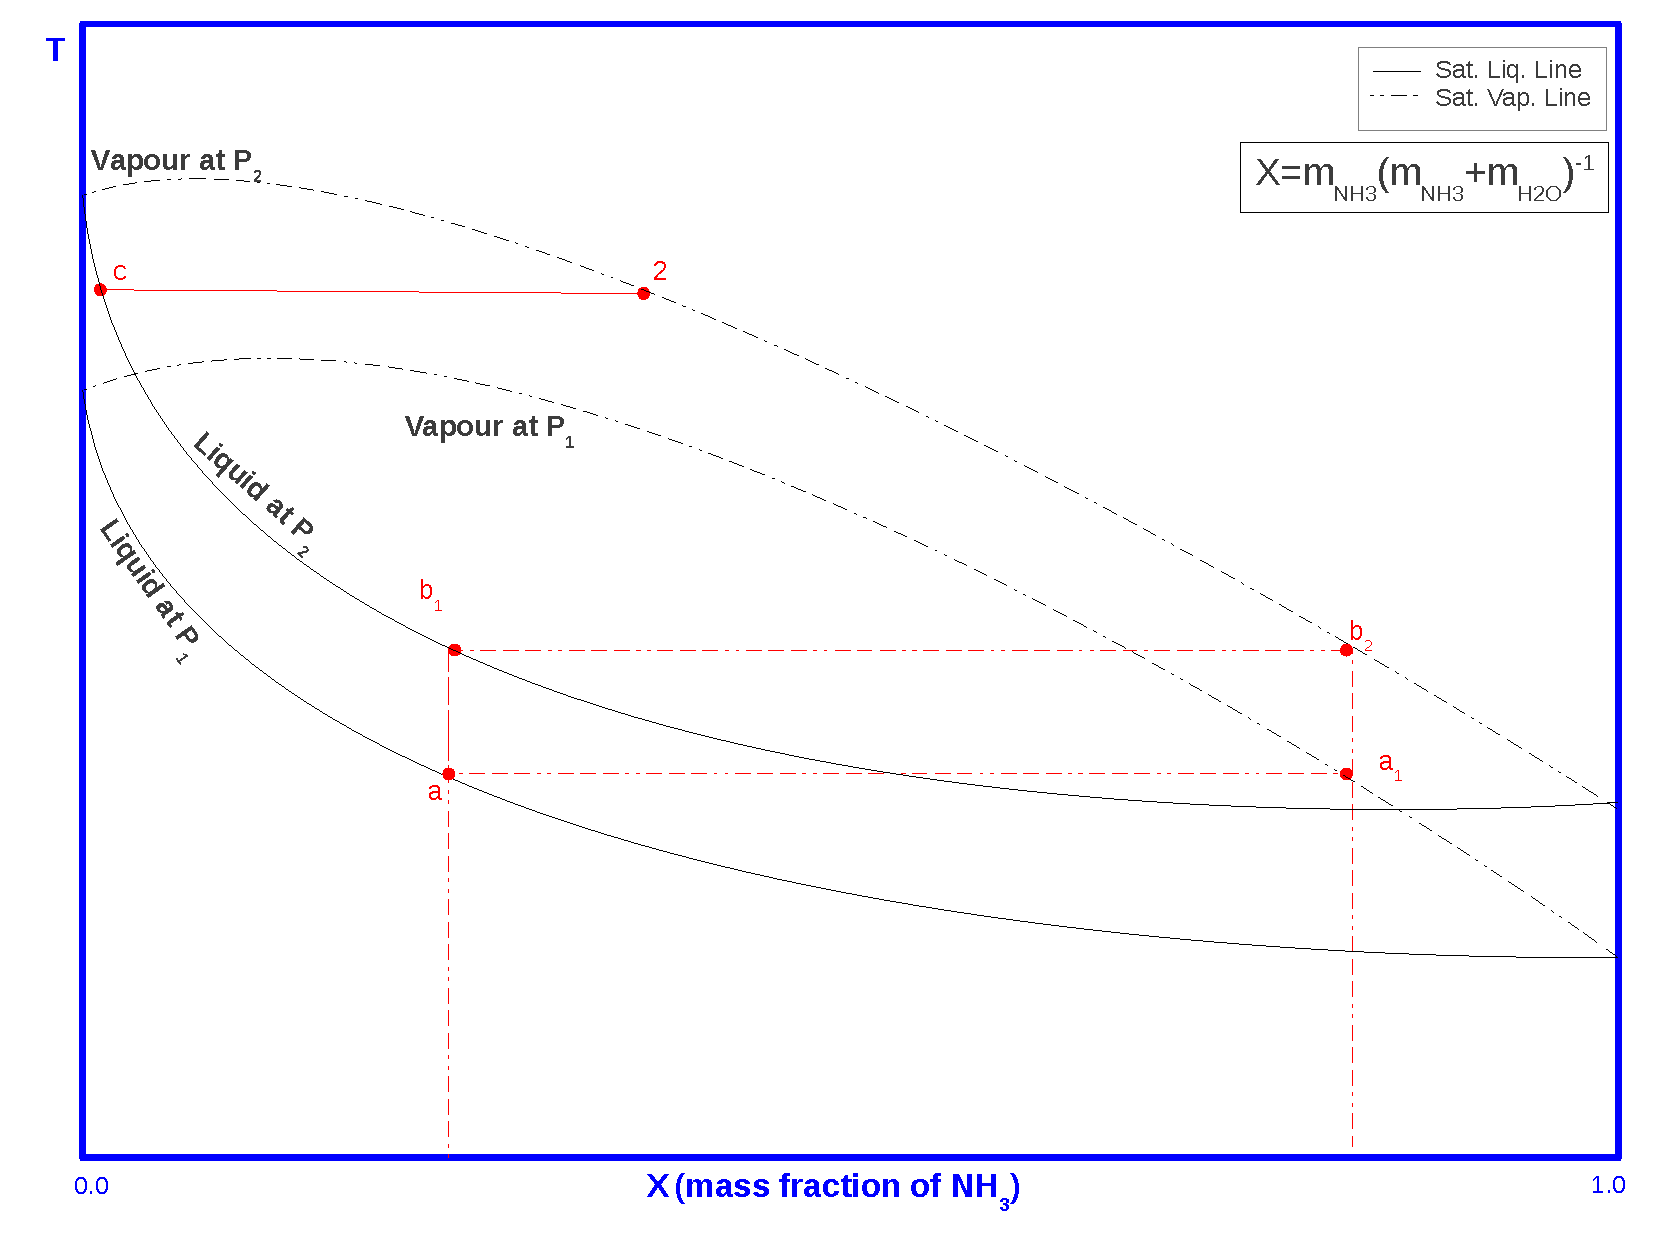
\includegraphics[width=5.5cm,height=5.cm,clip]{./Pics/Overview_Refrig34}
    \end{figure}  
   \end{column}  
   \begin{column}[c]{0.55\linewidth}
    \begin{enumerate}[(a)]
     \item <1-> Vapour-Liquid Equilibrium $\Longrightarrow$ $Tx$, $Px$ and $Hx$ diagrams;
     \item <2-> \textcolor{blue}{$x=1.0\;\Longrightarrow$} pure ammonia;
     \item <3-> Saturated liquid and saturated vapour can exist altogether $\left(P_{1}\right)$ in equilibrium as shown in states \textcolor{blue}{$a$} and \textcolor{blue}{$a_{1}$};
     \item <4-> The line \textcolor{red}{$a-a_{1}$} represents the vapour-liquid equilibrium (VLE) of $NH_{3}$ $\left(\text{at }P_{1}\right)$ with composition $x_{a}$ (liquid phase) and $x_{a1}$ (vapour phase) --- $x_{a1}>x_{a}$;
   \end{enumerate}
  \end{column}  
 \end{columns}  
\end{frame}

%%%
%%% Slide
%%%
\begin{frame}
 \frametitle{Basic Principles -- Phase Equilibrium Diagram} 
  \begin{columns}
   \begin{column}[c]{0.45\linewidth}
    \begin{figure}%
     \vbox{
      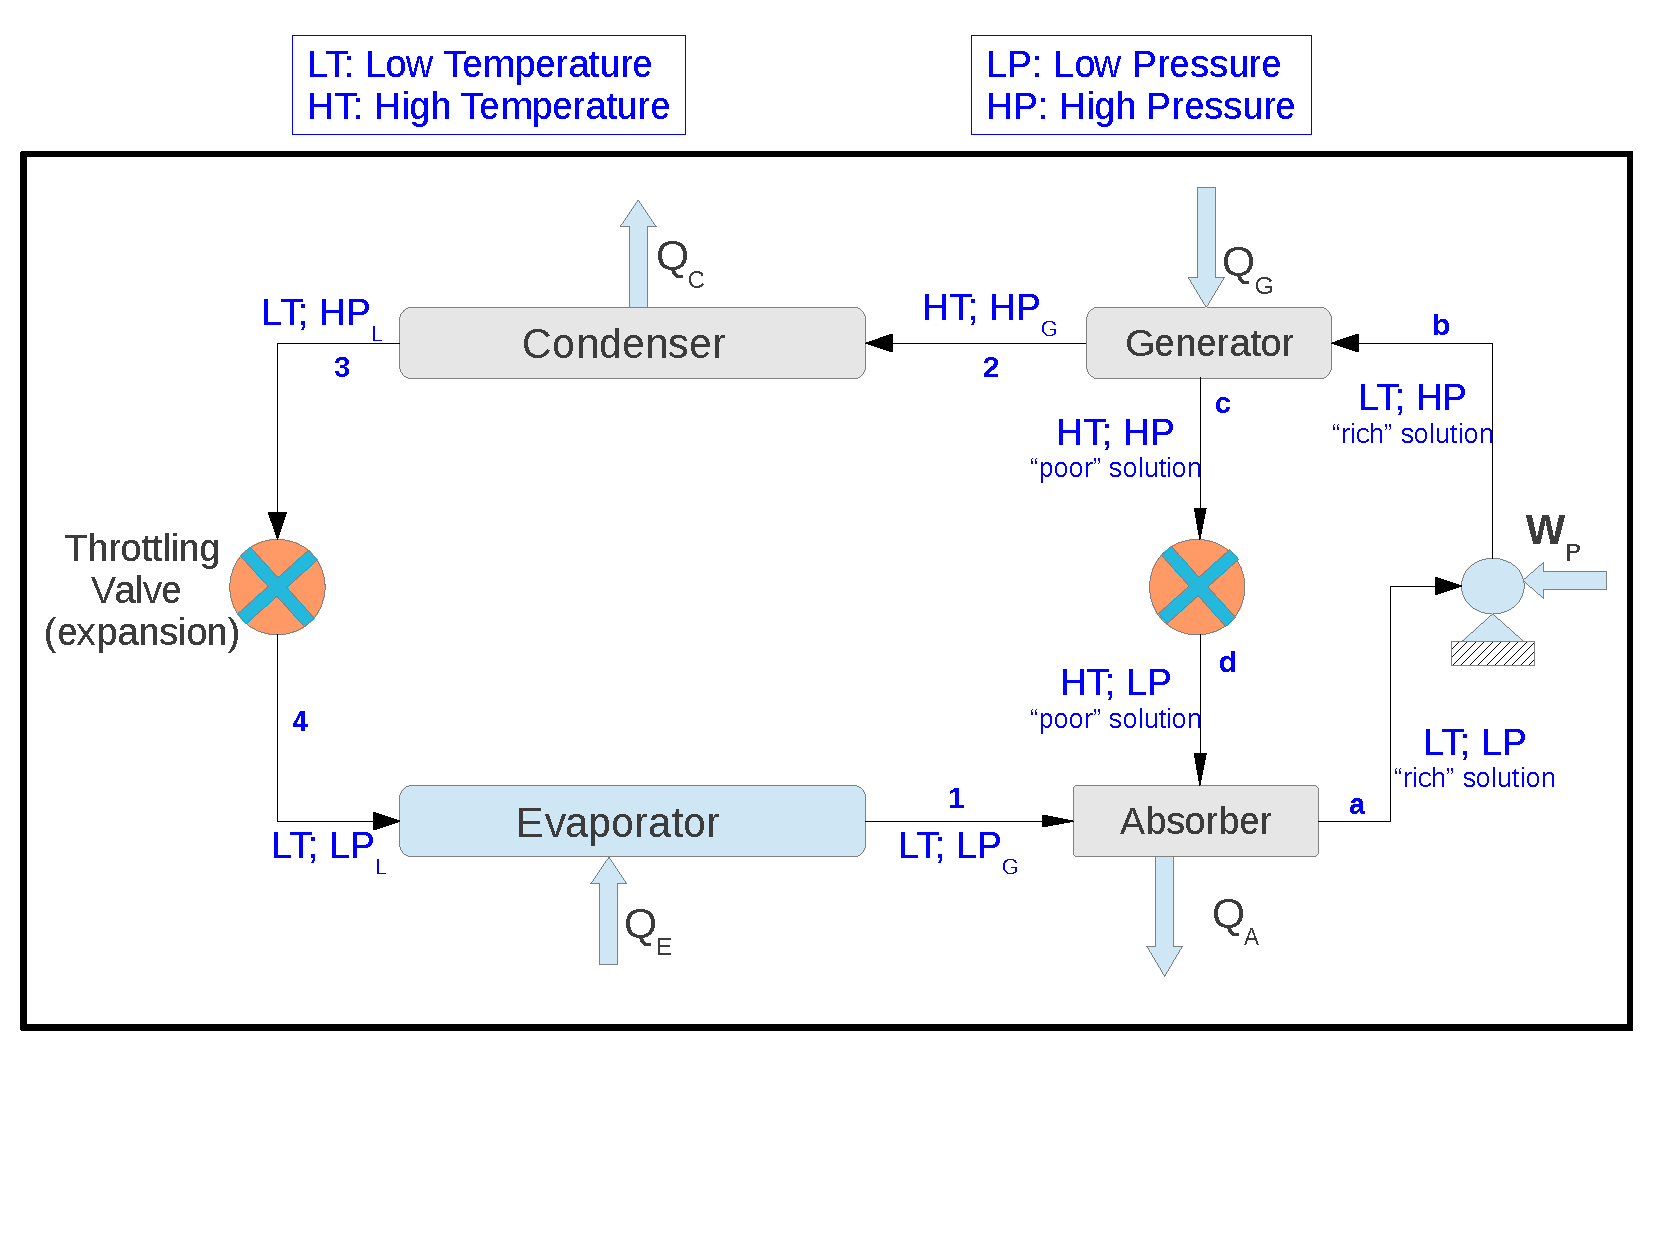
\includegraphics[width=4.5cm,height=4.cm,clip]{./Pics/Overview_Refrig32}
      \vspace{-.5cm}
      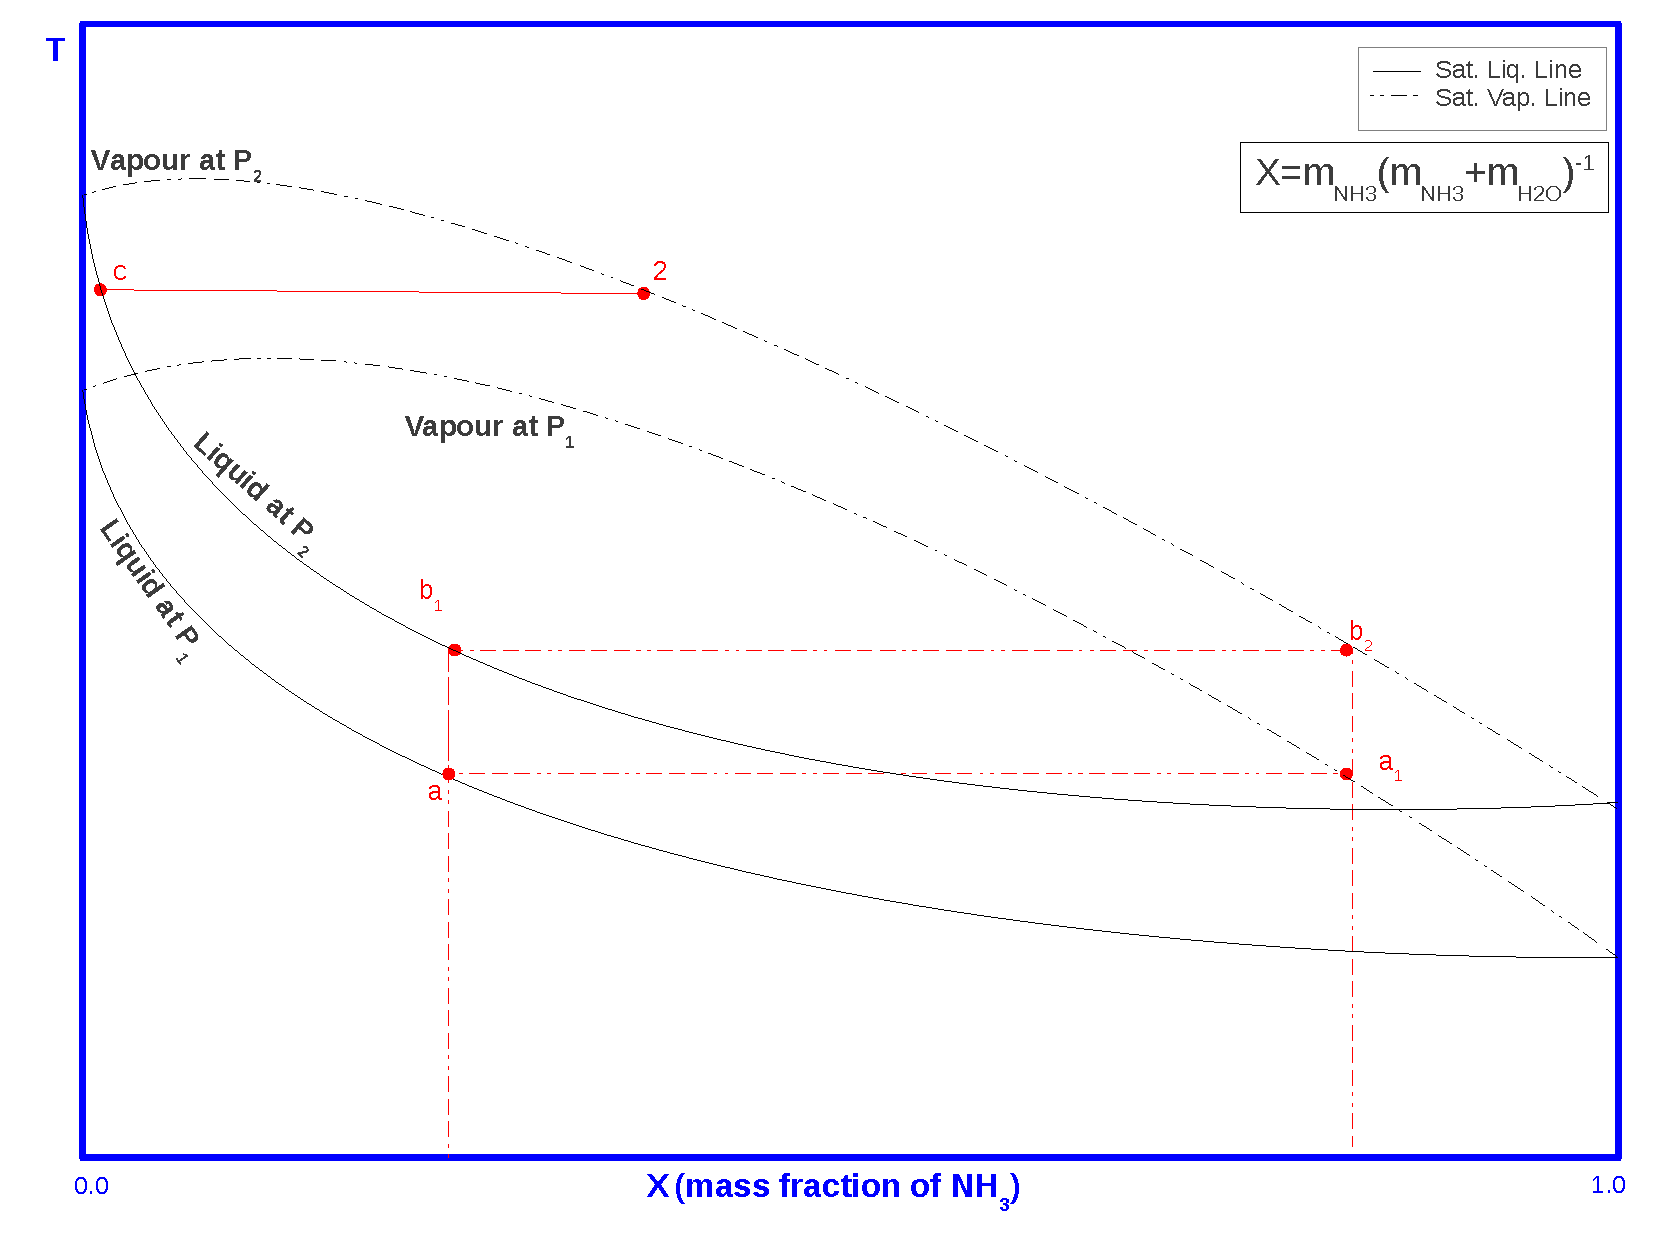
\includegraphics[width=4.5cm,height=4.cm,clip]{./Pics/Overview_Refrig34}}
    \end{figure}  
   \end{column}  
   \begin{column}[c]{0.55\linewidth}
    \begin{enumerate}[(a)]
     \item <1-> During the absorption cycle, $NH_{3}$ (vapour) from the {\it evaporator} is absorbed by the $H_{2}O$ releasing heat ({\it exothermic} dissolution);
     \item <2-> For $NH_{3}$ to be absorbed, the temperature needs to be low, and the heat is removed by using a recirculating cooling water in the {\it absorber};
     \item <3-> \textcolor{blue}{Saturated liquid} at state \textcolor{red}{$a$} leaves the {\it absorber} at $P_{1}$ and is driven into the {\it pump} where the pressure is raised to $P_{2}$;
     \item <4-> In order to evaporate the $NH_{3}$, the solution is heated in the {\it generator} ({\it endothermic} process);
   \end{enumerate}
  \end{column}  
 \end{columns}  
\end{frame}


%%%
%%% Slide
%%%
\begin{frame}
 \frametitle{Basic Principles -- Phase Equilibrium Diagram} 
  \begin{columns}
   \begin{column}[c]{0.45\linewidth}
    \begin{figure}%
     \vbox{
      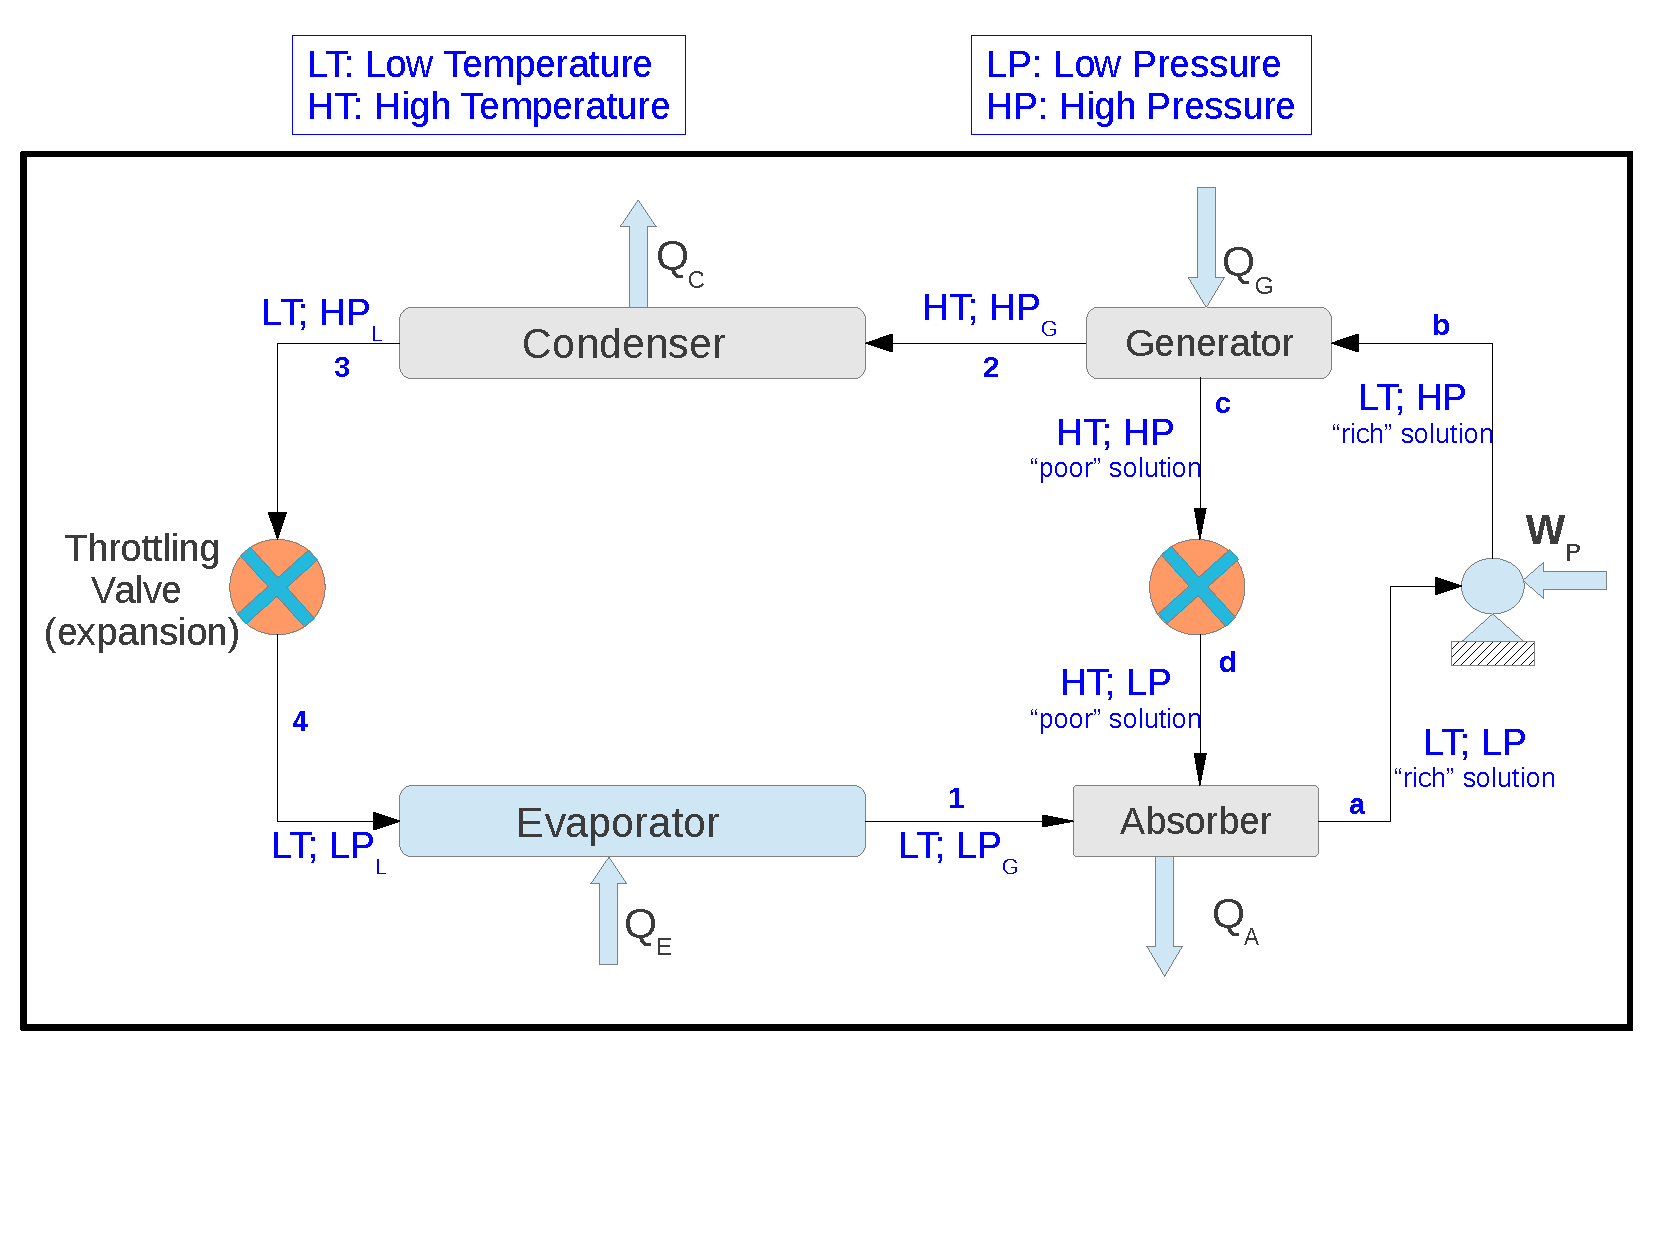
\includegraphics[width=4.5cm,height=4.cm,clip]{./Pics/Overview_Refrig32}
      \vspace{-.5cm}
      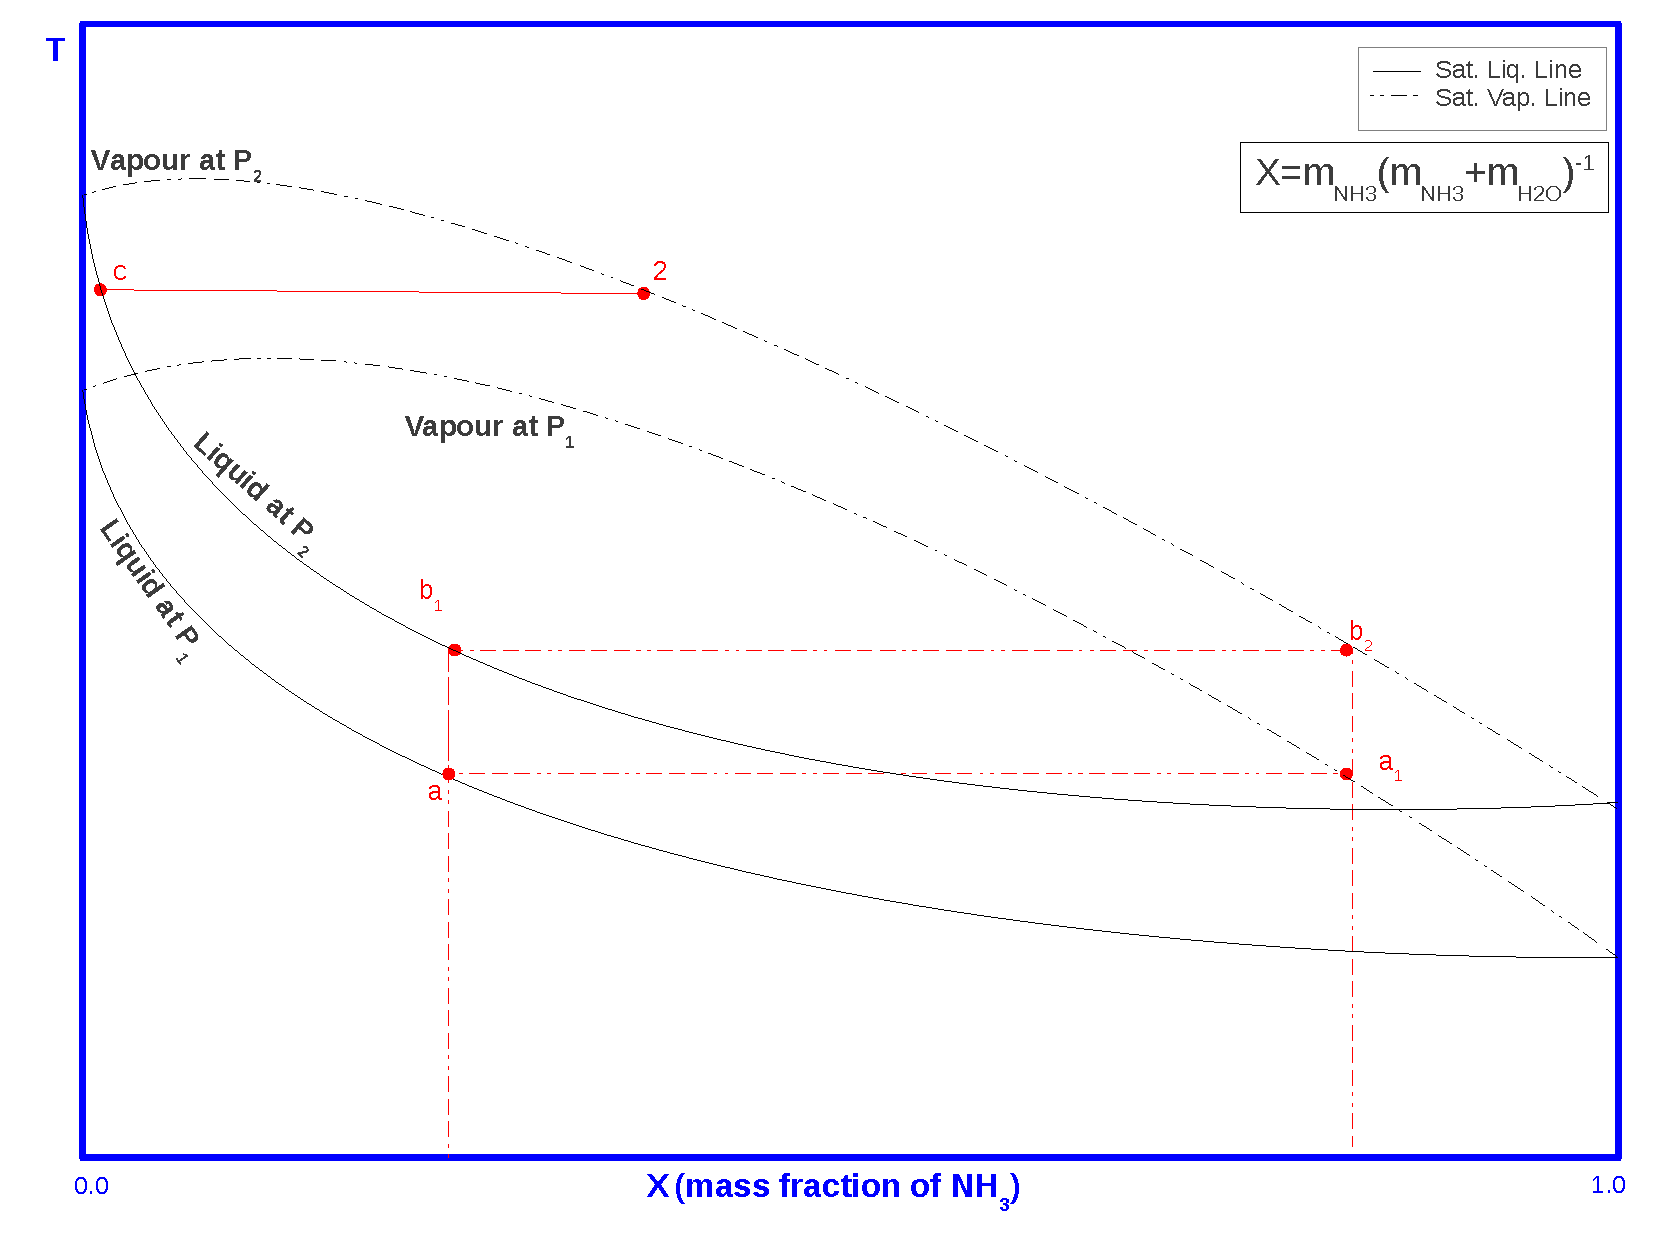
\includegraphics[width=4.5cm,height=4.cm,clip]{./Pics/Overview_Refrig34}}
    \end{figure}  
   \end{column}  
   \begin{column}[c]{0.55\linewidth}
    \begin{enumerate}[(a)]
     \item <1-> Further heat addition in the {\it generator} leads to the evaporation of the liquid $NH_{3}$ solution to a vapour of composition $x_{b2}$;
     \item <2-> Transformation from $b_{1}$ to $b_{2}$ leads to the formation of $NH_{3}$ rich vapour (thus with reduced concentration of ammonia liquid).
     \item <3-> If we keep $P$ and $T$ constant, the evaporation stops at low concentration liquid as it has not reached the boiling point;
   \end{enumerate}
  \end{column}  
 \end{columns}  
\end{frame}


%%%
%%% Slide
%%%
\begin{frame}
 \frametitle{Basic Principles -- Phase Equilibrium Diagram} 
  \begin{columns}
   \begin{column}[c]{0.45\linewidth}
    \begin{figure}%
     \vbox{
      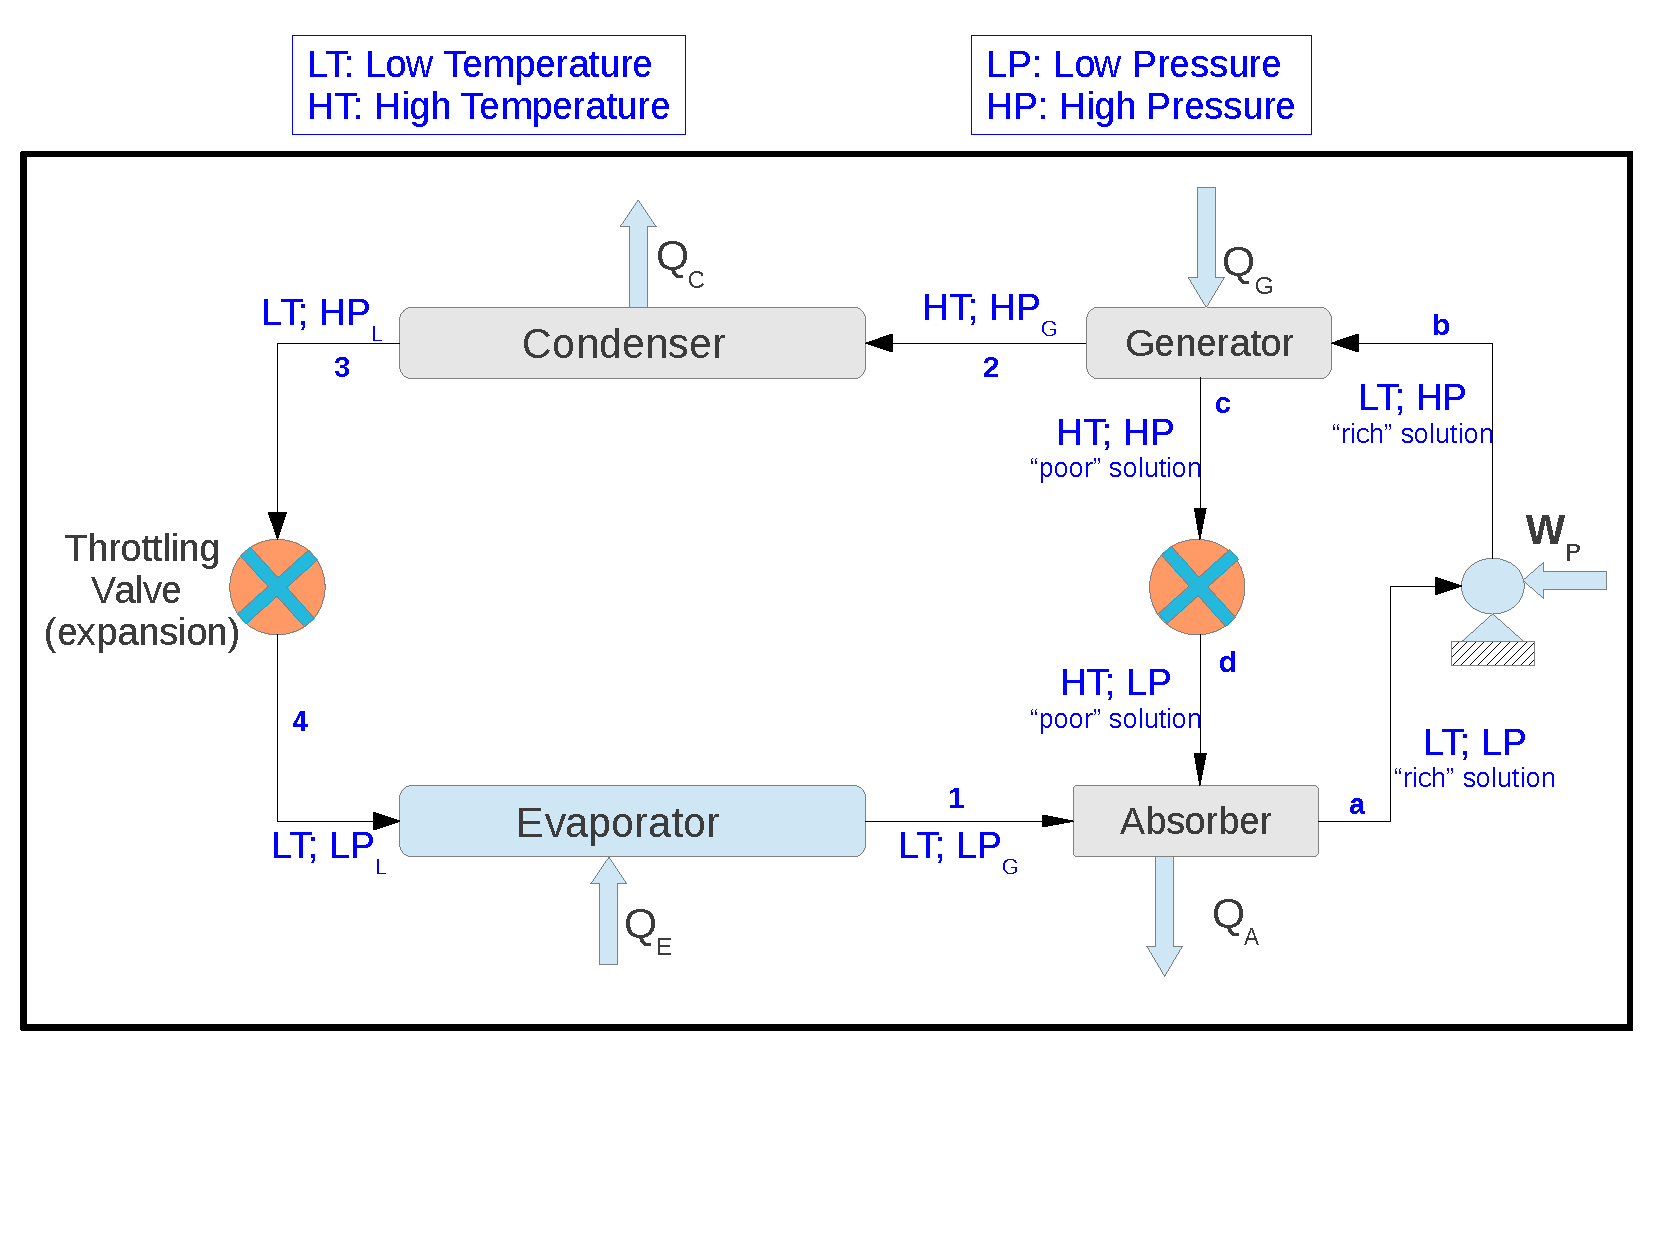
\includegraphics[width=4.5cm,height=4.cm,clip]{./Pics/Overview_Refrig32}
      \vspace{-.5cm}
      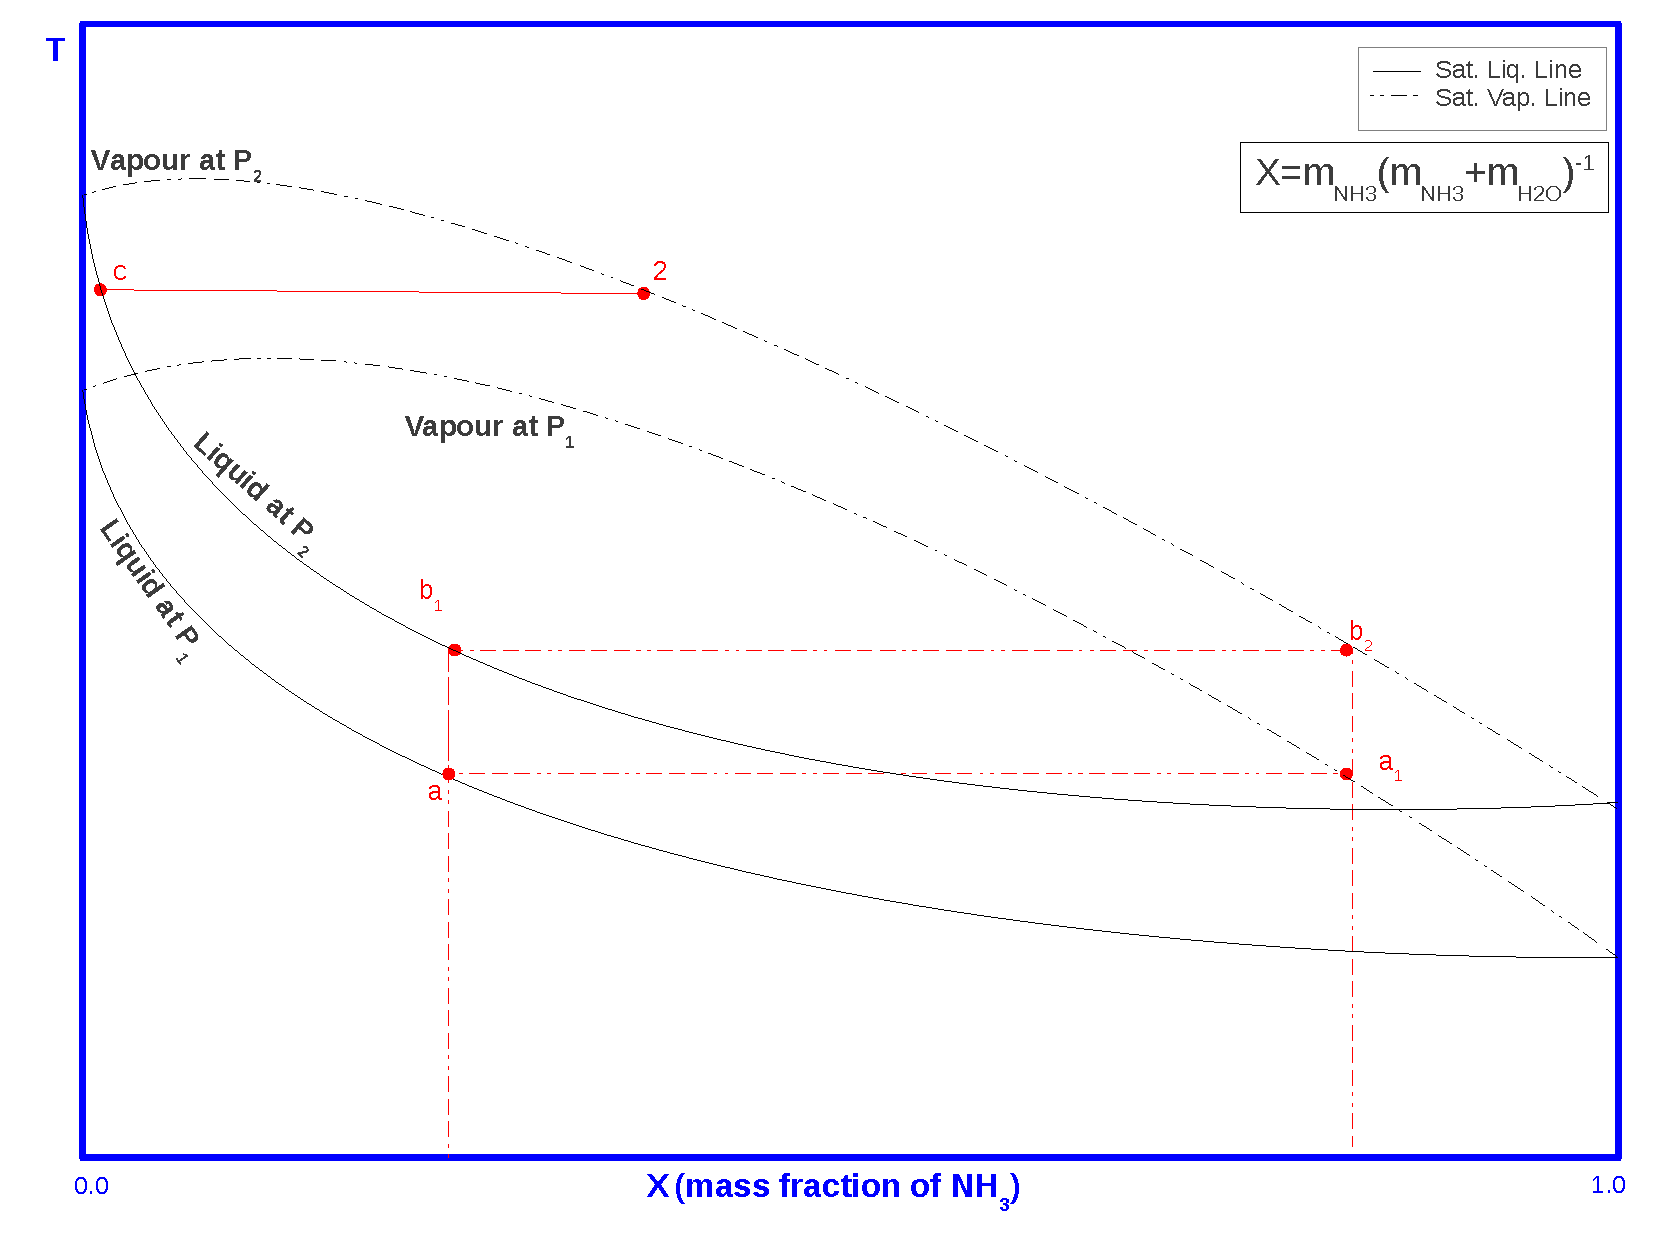
\includegraphics[width=4.5cm,height=4.cm,clip]{./Pics/Overview_Refrig34}}
    \end{figure}  
   \end{column}  
   \begin{column}[c]{0.55\linewidth}
    \begin{enumerate}[(a)]
     \item <1-> By adding further heat (in the generator), the evaporation continues and the mixture's temperature is raised with new liquid and vapour being formed as $c$ and $2$, respectively;
     \item <2-> Liquid at {\it c} is weak $NH_{3}+H_{2}O$ mixture and is driven back to the {\it absorber};
     \item <3-> $NH_{3}$ vapour leaves at state {\it 2} from the {\it generator} to the {\it condenser}.
   \end{enumerate}
  \end{column}  
 \end{columns}  
\end{frame}



%%%
%%% Slide
%%%
\begin{frame} 
 \frametitle{Basic Principles -- COP} 
    \begin{figure}%
      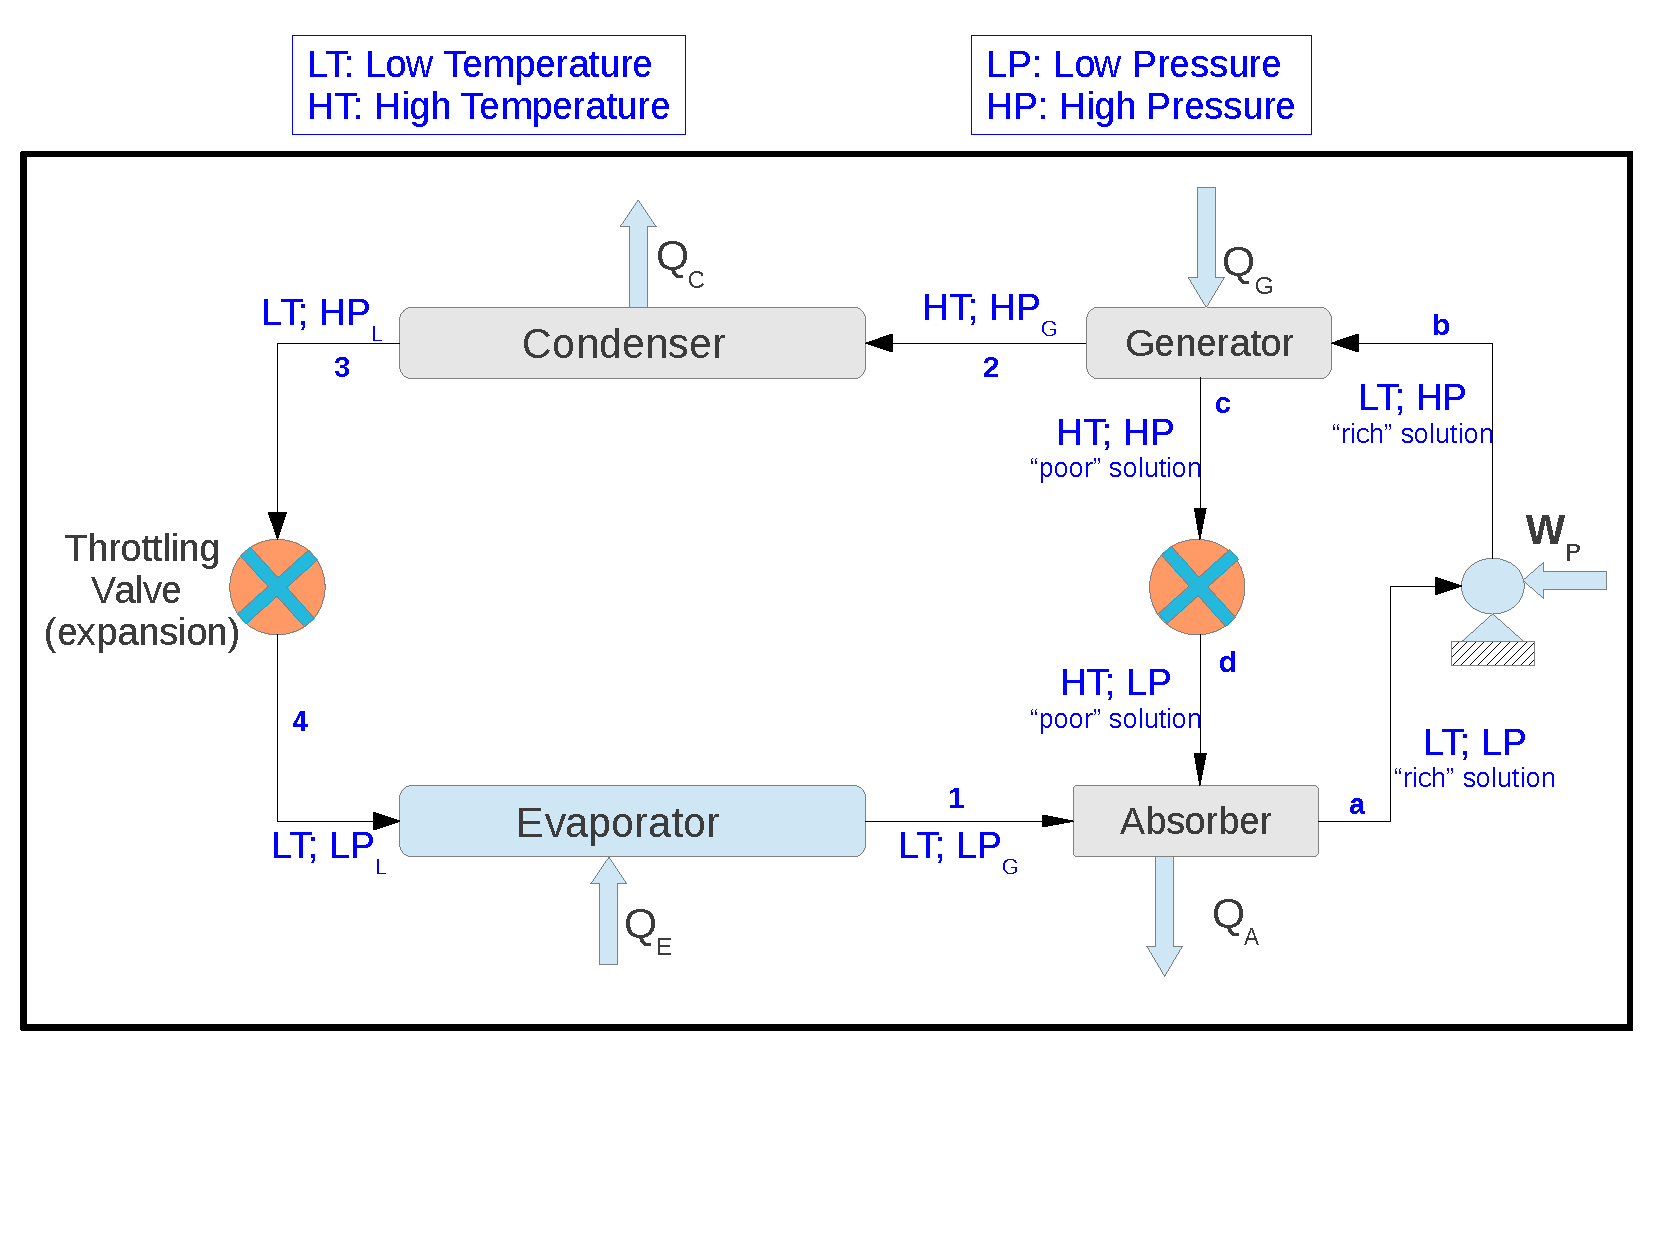
\includegraphics[width=6.5cm,height=4.cm,clip]{./Pics/Overview_Refrig32}
    \end{figure}  

   \begin{eqnarray}
    \textcolor{blue}{COP} &=& \frc{\text{Refrigerating Capacity}}{\text{Heat supplied in the generator}+\text{Work done by the liquid pump}} \nonumber \\
                          &=& \textcolor{blue}{\frc{Q_{E}}{Q_{G}+\dot{W}_{P}}} \nonumber   \\
                          && \textcolor{blue}{\text{(neglecting the work pump)}} \nonumber
   \end{eqnarray}
\end{frame}

%%%
%%% Slide
%%%
\begin{frame} 
 \frametitle{Desired Refrigerant-Absorbent Properties for VARCs} 
 \begin{enumerate}[(a)]
  \item <1-> High solubility of the refrigerant in the absorbent (Raoult's law) and small heat of solution;
  \item <2-> Large difference in the boiling temperature of the refrigerant and absorbent. This ensures that the refrigerant will be the {\it only} component to be evaporated and driven to the remaining of the refrigeration cycle (condenser -- expansion valve -- evaporator);
  \item <3-> The refrigerant-absorbent solution should exhibit high thermal conductivity and low viscosity;
  \item <4-> The refrigerant-absorbent solution should be safe, chemically stable, non-corrosive and inexpensive.
 \end{enumerate}
\end{frame}


\end{document}
